\documentclass[lineno]{jfm}

\usepackage{graphicx}
%\usepackage{epstopdf,epsfig}
\usepackage{newtxtext}
\usepackage{newtxmath}
\usepackage{natbib}
\usepackage{hyperref}
\usepackage{mathtools}
\usepackage{commath}
\usepackage{todonotes}

%
\usepackage[justification=justified]{caption}


\hypersetup{
    colorlinks = true,
    urlcolor   = blue,
    citecolor  = black,
}
\newtheorem{lemma}{Lemma}
\newtheorem{theorem}{Theorem}
\newtheorem{corollary}{Corollary}
\newcommand{\RomanNumeralCaps}[1]
\linenumbers


% Bryan's Marcros
\renewcommand{\aa}{\mathbf{a}}
\newcommand{\bd}{\partial}
\newcommand{\dd}{\mathbf{d}}
\newcommand{\DD}{\mathcal{D}}
\newcommand{\eeta}{\boldsymbol{\eta}}
\newcommand{\FF}{\mathbf{F}}
\newcommand{\GG}{\mathbf{G}}
\newcommand{\JJ}{\mathbf{J}}
\newcommand{\nnu}{\boldsymbol{\nu}}
\newcommand{\ttau}{\boldsymbol{\tau}}
\newcommand{\ssigma}{\boldsymbol{\sigma}}
\newcommand{\rr}{\mathbf{r}}
\newcommand{\RR}{\mathbf{R}}
\renewcommand{\SS}{\mathbf{S}}
\newcommand{\xx}{\mathbf{x}}
\newcommand{\XX}{\mathbf{X}}
\newcommand{\uu}{\mathbf{u}}
\renewcommand{\vv}{\mathbf{v}}
\newcommand{\yy}{\mathbf{y}}
\newcommand{\pderiv}[2]{\frac{\partial #1}{\partial #2}}
\newcommand{\jump}[1]{[\![ #1 ]\!]}
\newcommand{\ReviewerOne}[1]{\textcolor{red}{#1}}
\newcommand{\ReviewerTwo}[1]{\textcolor{green}{#1}}
\newcommand{\ReviewerThree}[1]{\textcolor{magenta}{#1}}


% {\MakeUppercase{\romannumeral #1}}

%\title{Two-Dimensional Vesicles Under External Flow via Integral Equation Method}
\title{Two-Dimensional Vesicle Hydrodynamics from Hydrophobic Attraction Potential}
%\title{Hydrodynamics of Amphiphilic Particles in Background Flows}
%\author{Alan N. Jones\aff{1}
%  \corresp{\email{JFMEditorial@cambridge.org}},
%  H.-C. Smith\aff{1}
% \and J.Q. Long\aff{2}}
%
%\affiliation{\aff{1}STM Journals, Cambridge University Press, The Printing House, Shaftesbury Road, Cambridge CB2 8BS, UK
%\aff{2}DAMTP, Centre for Mathematical Sciences, Wilberforce Road, Cambridge CB3 0WA, UK}


\author{
Szu-Pei Fu\aff{1},
Bryan Quaife\aff{2},
Rolf Ryham\aff{1}, \and
Yuan-Nan Young\aff{3}
}
 \affiliation{
\aff{1}Department of Mathematics, \\Fordham University, Bronx, New York 10458, USA
\aff{2}Department of Scientific Computing, \\Florida State University, Tallahassee, Florida 32306, USA
\aff{3}Department of Mathematical Sciences, New Jersey Institute of Technology,\\ Newark, New Jersey 07102, USA
 }





\begin{document}
\maketitle

\begin{abstract}
  We develop a new model, to our knowledge,  for the many-body  hydrodynamics of amphiphilic 
  Janus particles suspended in a viscous background flow. 
  The Janus particles interact through a hydrophobic attraction potential 
  that leads to self-assembly into bilayer structures.   
  We adopt an efficient integral equation method for solving the screened
  Laplace equation for hydrophobic attraction and 
  for solving the mobility problem for hydrodynamic interactions. 
  The integral equation formulation accurately captures both interactions for near touched boundaries. 
  Under a linear shear flow,  we observe the tank-treading deformation
  in a two-dimensional vesicle made of Janus particles.
  The results yield measurements of inter-monolayer friction, membrane permeability, 
  and at large shear rates, membrane rupture. 
  The simulations studies include a vesicle in parabolic flow and vesicle-vesicle 
  interactions in shear and extensional flows. The hydrodynamics of the Janus 
  particles vesicle replicate the behaviour of an inextensible elastic vesicle membrane.
%    We develop a new model, to our knowledge,  for the hydrodynamics of amphiphilic particles in background flows. 
%  In this work, we study the dynamics of many-body systems immersed in a
%  viscous fluid with a specified interparticle force. In particular, we
%  apply a hydrophobic attraction potential (HAP) using a Janus type
%  granular system to model lipid bilayer membranes. Coupling with an
%  efficient integral equation method for rigid bodies in Stokes flow and
%  a previous developed HAP solver, the deformations of a two-dimensional
%  vesicle such as tank-treading motion and membrane ruptures can be
%  observed under different values of the shear rate. Moreover, an
%  efficient integral equation method is adopted for solving the screened
%  Laplace equation and the mobility problem where it can accurately
%  calculate hydrophobic and hydrodynamic interactions between near
%  touched boundaries.
\end{abstract}


\begin{keywords}
Authors should not enter keywords on the manuscript, as these must be chosen by the author during the online submission process and will then be added during the typesetting process (see \href{https://www.cambridge.org/core/journals/journal-of-fluid-mechanics/information/list-of-keywords}{Keyword PDF} for the full list).  Other classifications will be added at the same time.
\end{keywords}

{\bf MSC Codes }  {\it(Optional)} Please enter your MSC Codes here



%%%%%%%%%%%%%%%%%%%%%%%%%%%%%%%%%%%%%%%%%%%%%%%%%%%%%%%%%%%%%%%%%%%%%%%
\section{\label{intro}Introduction}
Described by physicist Pierre-Gilles de Gennes as ``another animal in soft matter physics", the
Janus particle--often a spherical particle with a hydrophobic and a
hydrophilic hemisphere--exhibits complex aggregate, clustering, and
self-assembly into mesoscopic and macroscopic structures that are
relevant to a wide range of applications in biology and bioengineering (\cite{deGennes1991}).
Whether it is surface chemistry or polarity under an external field, the
dynamics of Janus particles in a viscous solvent is inevitably the combination of long-range
hydrodynamics interactions with both short- and intermediate-range 
particle-particle interactions. Such multi-scale nature of Janus particle dynamics underlies 
the richness of a Janus particle suspension, as \cite{deGennes1991} suggested by the example of 
a ``thin film of Janus grains" that can breathe due to the interstices between Janus particles.

\begin{figure}
\begin{center}
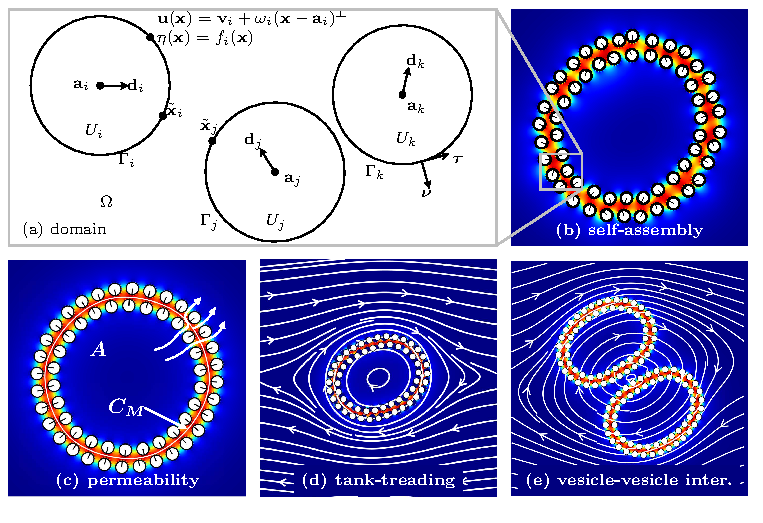
\includegraphics[width=\textwidth]{Figure0_Wrapper.pdf}
\end{center}
\caption{Panel (a) illustrates the domain and boundary conditions for
  the mobility problem. The color map in panels (b)--(e) is the solution
  $u$ of \eqref{eq:SL}. Red is for $u = 1$ and blue is for $u = 0$.
  Particles self-assemble into vesicle bilayers (panel (b)) and
  eventually arrange along inner and outer leaflets. In panel (c), $C_M$
  is the midplane curve, \ReviewerOne{and} $A$ is the enclosed area\ReviewerOne{.}
  %, and $L$ is the arc length. 
  Initially stretched vesicles relax to equilibrium with fluid
  flow across the bilayer. The study considers a single vesicle in
  background flows such as shear flow (panel (d)) and hydrodynamic
  vesicle-vesicle interactions (panel (e)).}
\label{fig:figure0}
\end{figure}

Recently,~\cite{Fu20} illustrated that the hydrophobic interactions
between Janus particles (JP) in a viscous solvent can be used as a
coarse-grained model to capture the mechanics of an elastic bilayer
membrane of amphiphilic macromolecules such as lipids. Depending on
their total number and geometry, JP suspensions can aggregate to form a
micelle, a patch of bilayer membrane with open ends, and a self-enclosed
bilayer membrane, referred to as a JP vesicle. Using a hybrid continuum
model for the interactions between amphiphilic particles in a viscous
solvent and with a boundary integral formulation,~\cite{Fu20} showed
that the granularity of membrane remodeling, as occurs during fusion and
fission of bilayers, can be accurately captured by the coarse-grained
model.  
%This boundary integral formulation has inspired more recent work

In the present work, we extend the hybrid continuum model in~\cite{Fu20}
for the Janus suspension to incorporate the collective hydrodynamics of
a Janus suspension under various flows. The JP vesicles in our
simulations replicate  \ReviewerOne{well-known} vesicle hydrodynamics
such as tank-treading and inter-leaflet slippage in a shear flow and
migration in Poiseuille flow from continuum models. Furthermore we use
the hybrid continuum model to investigate permeability and rupture of a
bilayer membrane due to an imposed flow.  Finally, we compare a pair of
interacting JP vesicles with a continuum model of a pair of vesicles.

\cite{Brandner2019} used the coarse-grained force field with a lattice
Boltzmann molecular dynamics to simulate the hydrodynamics of a
nano-sized vesicle under a shear flow.  In MD simulations, the
hydrodynamic interactions for the solvent phase are often approximated
by an implicit solvent coarse-grained model.  In the present work, the
hydrodynamic interactions come from the mobility problem for the Stokes
equations for the incompressible, viscous solvent.  

We require a numerical method to avoid unphysical contact between rigid
Janus particles. Optimization-based contact methods introduce
constraints, such as enforcing a non-positive space-time interference
volume (\cite{lu-rah-zor2017, Lukas19, yan-cor-mal-vee-she2020}). These
methods do not introduce stiffness, but do require solving potentially
expensive nonlinear complementarity problems at each time step.
Repulsion-based contact methods, which we employ, introduce an
artificial repulsion force that increases in strength as two particles
approach one another (\cite{glo-pan-hes-jos-per2001, fen-mic2004,
kab-qua-bir2018}). Strong repulsion forces can introduce numerical
stiffness, but with the presence of the hydrophobic forces, we maintain
contact-free suspensions with a relatively weak non-stiff repulsive
force.

The paper is organized as follows. In \S~\ref{sec:governing_eqs} we
present the formulation for the Janus particles in a viscous fluid in
the zero-Reynolds number regime (Figure \ref{fig:figure0}a). In
\S~\ref{sec:IEM} we extend the hybrid continuum model for a Janus
suspension to include the effects of a far-field flow via the mobility
problem formulation. In \S~\ref{results} we validate our model and
present simulation results for a single JP vesicle (Figure
\ref{fig:figure0}d) and for a pair of JP vesicles (Figure
\ref{fig:figure0}e) under various flowing conditions. Finally we provide
discussion and outlook for future directions in \S~\ref{conclusion}.

%%%%%%%%%%%%%%%%%%%%%%%%%%%%%%%%%%%%%%%%%%%%%%%%%%%%%%%%%%%%%%%%%%%%%%%


\section{Governing Equations\label{sec:governing_eqs}}
\subsection{\label{mobility}Mobility Problem}
The objective of this work is to study the hydrodynamics of JP vesicles
in background flows. We consider an $N_b$-many body collection of JP
suspended in a two-dimensional unbounded domain $\Omega$. The boundary
of each particle is denoted by $\Gamma_i$ so that $\bd \Omega = \Gamma_1
\cup \Gamma_2 \cup \cdots \cup \Gamma_{N_b}$ (Figure
\ref{fig:figure0}a). Assuming the inertial terms are negligible, the
governing equations are
\begin{alignat}{3}
\label{eq:stokes}
  -\mu \Delta \uu + \nabla p &= \mathbf{0}, 
    && \xx \in \Omega, \\
  \nabla\cdot \uu &= 0, \qquad && \xx \in \Omega, \\
  \uu - \uu_\infty &\to \mathbf{0}, && |\xx| \to \infty,
\end{alignat}
%
where $\uu$ is the velocity, $p$ is the
pressure, $\uu_\infty$ is the background flow, and $\mu$ is the constant viscosity. 
%
Since each particle $\Gamma_i$ with centre $\aa_i$ is a rigid body, its velocity satisfies 
\ReviewerOne{the no-slip boundary condition}
\begin{align}
  \ReviewerOne{\uu}(\xx) = \vv_i + \omega_i (\xx - \aa_i)^\perp, \quad 
    \xx \in \Gamma_i,
\end{align}
where $\vv_i$ is its translational velocity and $\omega_i$ is its
angular velocity. Here, $\langle x, y \rangle^{\perp} = \langle -y, x
\rangle$.
%Therefore, the no-slip boundary condition on each particle is
%
%
%\begin{align}
%\label{eq:rigid_bc}
%  \uu(\xx) = \vv_i + \omega_i (\xx - \aa_i)^\perp, \quad
%    \xx \in \Gamma_i.
%\end{align}
%
%
To determine the translational and angular velocities of each particle,
we define imposed forces $\FF_i$ and torques $T_i$ acting on each
particle. Since the small particles are inertialess, force and torque
balance gives 
\begin{alignat}{2}
  \label{eq:force}
  \FF_i &- \int_{\Gamma_i} \ssigma \cdot \nnu \, \dif s = \mathbf{0},
  && i=1,\ldots,N_b,\\
  \label{eq:torque}
  T_i &- \int_{\Gamma_i} (\xx - \aa_i)^\perp \cdot 
    (\ssigma \cdot \nnu) \, \dif s = 0, \qquad && i=1,\ldots,N_b,
\end{alignat}
where $\ssigma = -p \mathbf{I} + \mu \left(\nabla \uu + \nabla \uu^T
\right)$ is the hydrodynamic stress tensor (pressure tensor) and
$\nnu$ is the particle outward normal. The process of finding the
translational and angular velocities given the forces and torques is
referred to as the mobility problem.


%%%%%%%%%%%%%%%%%%%%%%%%%%%%%%%%%%%%%%%%%%%%%%%%%%%%%%%%%%%%%%%%%%%%%%%
\subsection{Imposed Forces}
The imposed forces and torques contain two parts: hydrophobic attraction
and repulsion. The hydrophobic attraction potential was introduced
by~\cite{Fu20} and is responsible for forming particle aggregates that
sequester their hydrophobic surface regions (Figure \ref{fig:figure0}b).
We model hydrophobic attraction by solving the screened Laplace equation
boundary value problem
\begin{alignat}{2}
  \label{eq:SL}
-\rho^2 \Delta u + u &=0,            && \xx \in \Omega,\\
\label{eq:SLbc}
u(\xx) &= f_i(\xx),\qquad  && \xx \in \Gamma_i,\; i=1,\ldots,N_b, \\
\label{eq:SLff}
u &\to 0,                          &&|\xx| \to \infty,
\end{alignat}
where $0 \leq f_i \leq 1$ is a material label with $f_i = 0$,
respectively $1$, representing hydrophilic, respectively hydrophobic,
portions of the surface. We assume that both $f_i$ and $\Gamma_i$ are
smooth. The parameter $\rho > 0$ is the decay length of attraction. The
forces and torques of attraction are 
\begin{align}
  \label{eq:hydrophobicAttraction}
  \FF_i^{\text{hydro}} = \int_{\Gamma_i} {\bf T}\cdot \nnu \, \dif s, 
    \quad 
  T_i^{\text{hydro}} = \int_{\Gamma_i} (\xx - \aa_i)^{\perp} \cdot ({\bf T} \cdot \nnu) \dif s,
\end{align}
where
\begin{align}
  \label{eq:stress}
\mathbf{T}
= \gamma\rho^{-1}u^2 \mathbf{I} + 2\rho\gamma \left(\tfrac{1}{2}|\nabla
  u|^2 \mathbf{I} - \nabla u  \nabla u^T\right)
\end{align}
is the hydrophobic stress tensor and $\gamma > 0$ is
the interfacial
tension. 

The second part of the imposed forces and torques comes from repulsion
between proximal particles. Given a pair particles indexed with $i$ and
$j$, we find the two points $\tilde{\xx}_i \in \Gamma_i$ and
$\tilde{\xx}_j \in \Gamma_j$ that are closest to one another (Figure \ref{fig:figure0}a). We then
define the repulsion force and torque
\begin{align}
  \label{eq:REPULforce}
  \FF_i^{\text{repul}} &= \sum_{j \neq i} 
    \frac{\tilde{\xx}_i - \tilde{\xx}_j}
    {|\tilde{\xx}_i - \tilde{\xx}_j|} 
    P'(|\tilde{\xx}_i - \tilde{\xx}_j|), \\
  \label{eq:REPULtorque}
  T_i^{\text{repul}} &= \sum_{j \neq i} 
    (\tilde{\xx}_i - \aa_i)^{\perp} \cdot 
    \frac{\tilde{\xx}_i - \tilde{\xx}_j}
    {|\tilde{\xx}_i - \tilde{\xx}_j|} 
    P'(|\tilde{\xx}_i - \tilde{\xx}_j|).
\end{align}
The repulsion profile $P(r)$ is set to zero for distances $r$ larger than a
repulsion length scale $\rho_0$. As such,~\eqref{eq:REPULforce}
and~\eqref{eq:REPULtorque} ignore particles outside a
$\rho_0$-tubular neighborhood of $\Gamma_i$. For $0 \leq r < \rho_0,$ we use
$P(r) = M(1 - \sin(r/\rho_0))$ where $M$ is sufficiently large to
prevent particle collisions. Then, the total imposed force and torque
are
\begin{equation}
\label{eq:total_forces}
  \FF_i = \FF_i^{\text{hydro}} + \FF_i^{\text{repul}},\quad
  T_i = T_i^{\text{hydro}} + T_i^{\text{repul}}, \qquad
  i=1,\ldots,N_b.
\end{equation}


%%%%%%%%%%%%%%%%%%%%%%%%%%%%%%%%%%%%%%%%%%%%%%%%%%%%%%%%%%%%%%%%%%%%%%%

%%%% moved to new section 3.4

%\subsection{Time Marching}
%By solving the mobility problem, we obtain translational and angular
%velocities of the $N_b$-body system. 
%A second-order Adams-Bashforth
%scheme updates the particle positions and orientations. By including the
%repulsion force~\eqref{eq:REPULforce}, particle collisions are avoided even
%when using a relatively large time step. 



%This paper is organized as follows. Chapter 2 introduces the mobility problem..... The integral equation method for solving $N_b$-body system with details of .... are included in Chapter 3. We provide numerical results of vesicle simulations in Chapter 4. Finally, we conclude the work and briefly give the picture of our future work.



%%%%%%%%%%%%%%%%%%%%%%%%%%%%%%%%%%%%%%%%%%%%%%%%%%%%%%%%%%%%%%%%%%%%%%%
\section{Integral Equation Method}
\label{sec:IEM}
Computing the hydrophobic attraction potential and the particle forces
and torques requires the solution of elliptic partial differential
equations (PDEs) in an unbounded complex domain. We recast both these
PDEs as boundary integral equations (BIEs). We discretize each BIE at
$N$ points on each of the $N_b$ particles with a collocation method.
\ReviewerOne{All derivatives are computed with spectrally-accurate
Fourier differentiation.} Integrals that are smooth are computed with
the spectrally-accurate trapezoid rule, and nearly-singular integrals,
caused by close contact between two particles, are computed with a
high-order interpolation-based quadrature rule (\cite{qua-bir2014}).
After discretizing and applying quadrature, the resulting linear system
is solved with matrix-free GMRES, and we guarantee that the number of
GMRES iterations is mesh-independent by using second-kind BIEs.


%%%%%%%%%%%%%%%%%%%%%%%%%%%%%%%%%%%%%%%%%%%%%%%%%%%%%%%%%%%%%%%%%%%%%%%
\subsection{HAP Boundary Integral Equation}
Similar to our previous work (\cite{Fu20}), we represent the
\ReviewerTwo{hydrophobic attraction potential (HAP)} as a double-layer
potential
\begin{align}
  \label{eq:HAP_DLP}
  u(\xx) = \frac{1}{2\pi} \int_{\bd\Omega} \left(\pderiv{}{\nnu_\yy}
    K_0 \left(\frac{|\xx - \yy|}{\rho}\right)\right) 
    \sigma(\yy) \, \dif s_\yy, \quad \xx \in \Omega,
\end{align}
where $K_0$ is the zeroth-order modified Bessel function of the first
kind and the integral is taken in the sense of principle value whenever
$\xx \in \partial \Omega$.  By requiring that the density function
$\sigma$ satisfies the second-kind integral equation
\begin{equation}
\label{eq:screenedSKIE}
  f(\xx) = \frac{1}{2}\sigma(\xx) + 
    \frac{1}{2\pi}\int_{\bd\Omega} \left(\pderiv{}{\nnu_\yy}
    K_0 \left(\frac{|\xx - \yy|}{\rho}\right)\right) \sigma(\yy) \, 
    \dif s_\yy, \quad \xx \in \bd\Omega,
\end{equation}
the HAP double-layer potential~\eqref{eq:HAP_DLP} satisfies the screened
Laplace equation~\eqref{eq:SL}--\eqref{eq:SLff}. After
discretizing~\eqref{eq:screenedSKIE}, the result is an $NN_b \times
NN_b$ linear system that is solved with block-diagonal preconditioned
GMRES.

To calculate the hydrophobic force and torque, the gradient of the
double-layer potential~\eqref{eq:HAP_DLP} must be computed on the
boundary of each particle. The resulting integrands are singular, and
specialized quadrature would be necessary to approximate such integrals.
Alternatively, in Section~\ref{subsec:calculating_force}, we show how
the force and torque calculations can be expressed in terms of
non-singular integrals.

%%%%%%%%%%%%%%%%%%%%%%%%%%%%%%%%%%%%%%%%%%%%%%%%%%%%%%%%%%%%%%%%%%%%%%%
\subsection{Mobility Problem Boundary Integral Equation}
Following previous work of~\cite{Lukas19}, we use the velocity
representation of~\cite{pow-mir1987}. In particular, we write the
velocity as the sum of a double-layer potential and $N_b$-many Stokeslets and
rotlets
\begin{align}
  \label{eq:velocity}
  \uu(\xx) = \uu_\infty(\xx) + \DD[\eeta](\xx) + 
    \sum_{i=1}^{N_b} \left(\SS(\xx,\aa_i) \cdot \FF_i + 
    \RR(\xx,\aa_i) T_i\right), \quad \xx \in \Omega.
\end{align}
The double-layer potential is
\begin{align}
  \DD[\eeta](\xx) = \frac{1}{\pi} \int_{\bd\Omega} 
    \frac{\rr \cdot \nnu}{|\rr|^2} \frac{\rr \otimes \rr}{|\rr|^2}
    \cdot \eeta(\yy) \, \dif s_\yy,
\end{align}
where $\rr = \xx - \yy$. The Stokeslet and rotlets centred at $\aa_i$
are
\begin{align}
  \SS(\xx,\aa_i) \cdot \FF_i &= \frac{1}{4\pi} \left(-\log |\rr| + 
    \frac{\rr \otimes \rr}{|\rr|^2}\right) \cdot \FF_i, \\
  \RR(\xx,\aa_i) T_i &= \frac{1}{4\pi} \frac{\rr^\perp}{|\rr|^2} T_i,
\end{align}
respectively, where $\rr = \xx - \aa_i$. The Stokeslet is torque-free
and has force $\FF_i$ while the rotlet is force-free and has torque
$T_i$. Therefore, the velocity~\eqref{eq:velocity} satisfies the total
force~\eqref{eq:force} and torque~\eqref{eq:torque} conditions if the
double-layer potential $\DD[\eeta]$ is force- and torque-free.  Matching
the limit of~\eqref{eq:velocity} with the rigid body motion, and
imposing that $\DD[\eeta]$ is force- and torque-free, the density
function $\eeta$, translational velocity $\vv_i$, and angular velocity
$\omega_i$ satisfy
\begin{alignat}{3}
  \nonumber
  \vv_i + \omega_i (\xx - \aa_i)^\perp &= \uu_\infty(\xx)
    -\frac{1}{2} \eeta(\xx) + \DD[\eeta](\xx) \\
  \label{eq:SKIE}
    + \sum_{j=1}^{N_b} &
    \left(\SS(\xx,\aa_j) \cdot \FF_j + \RR(\xx,\aa_j) T_j\right),
    \quad &&\xx \in \Gamma_i,\: i=1,\ldots,N_b, \\
  \label{eq:mobility1}
  \int_{\Gamma_i} \eeta \cdot \nnu \, \dif s &= {\bf 0}, 
  &&i = 1,\ldots,N_b, \\
  \label{eq:mobility2}
  \int_{\Gamma_i} \eeta\times(\xx-\aa_i)^\perp \cdot \nnu \, \dif s &= 0,
  &&i = 1,\ldots,N_b.
\end{alignat}

After discretizing and applying appropriate quadrature rules, the result
is a $(2NN_b + 3N_b) \times (2NN_b + 3N_b)$ linear system that we solve
with block-diagonal preconditioned GMRES. Other BIE formulations of the
mobility problem use single-layer potentials (\cite{cor-gre-rac-vee2017,
rac-gre2016}) or a combination of single- and double-layer potentials
(\cite{cor-vee2018}).

We have validated our solver for~\eqref{eq:SKIE}--\eqref{eq:mobility2}
using a single elliptical particle suspended in a background shear flow
(see \S~\ref{sec:ves_in_shear}). Hydrophobic attraction and repulsion
are zero for a single particle (see \cite{Fu20} equation 2.13). The
angle of the ellipse's major axis coming from the integral equation
method agrees with the theoretical, Jeffery orbit time-course
(\cite{jef1922}). 
  
%The Jeffrey orbit  
%\begin{equation}
%\label{eq:jeff}
%\Theta(t) = \tan^{-1}\left(\frac{a}{b}\tan \left(\frac{ab \dot\gamma t}{a^2+b^2}\right)\right)
%\end{equation}
%gives the angle between the major axis and $\mathbf{e}_2$
%where $a$, $b$ are the semi-major and semi-minor axes. 
%We are assuming $\Theta(0) = 0$.
% 

%The background flow is a shear flow $\uu_{\infty}(\xx) = \dot\gamma  \xx \cdot \mathbf{e}_2 \mathbf{e}_1$ with shear rate $\dot\gamma$
%and orthogonal unit vectors $\mathbf{e}_1$ and $\mathbf{e}_2$. 
%A single elliptical particle is suspended in the fluid with center at the origin.
%The Jeffrey orbit  
%\begin{equation}
%\label{eq:jeff}
%\Theta(t) = \tan^{-1}\left(\frac{a}{b}\tan \left(\frac{ab \dot\gamma t}{a^2+b^2}\right)\right)
%\end{equation}
%gives the angle between the major axis and $\mathbf{e}_2$
%where $a$, $b$ are the semi-major and semi-minor axes. 
%We are assuming $\Theta(0) = 0$.
%Figure~\ref{figure1} shows that the angles coming from the integral equation method \eqref{eq:SKIE}-\eqref{eq:mobility2}
%are in complete agreement with the theoretical time course \eqref{eq:jeff}.  Hydrophobic attraction and repulsion are zero for a single particle. 

%%%%%%%%%%%%%%%%%%%%%%%%%%%%%%%%%%%%%%%%%%%%%%%%%%%%%%%%%%%%%%%%%%%%%%%
\subsection{Main Theoretical Result: Calculating the Hydrophobic Force}
\label{subsec:calculating_force}
Once \eqref{eq:screenedSKIE} has been solved for $\sigma$, we need to
evaluate the integrals~\eqref{eq:hydrophobicAttraction} which are the
HAP forces and torques. These integrals involve the
stress~\eqref{eq:stress} which contains a singular integral for the
gradient of the double-layer potential. To avoid singular integrals, we
first define
\begin{align}
  \label{eq:uidef}
  w_i(\xx) = u(\xx) - u_i(\xx),
\end{align}
where
\begin{align}
  u_i(\xx) &= \frac{1}{2\pi} \int_{\Gamma_i} \left(\pderiv{}{\nnu_\yy}
    K_0 \left(\frac{|\xx - \yy|}{\rho}\right)\right) 
    \sigma(\yy) \, \dif s_\yy, \quad \xx \in \mathbb{R}^2.
\end{align}
That is, $w_i(\xx)$ is the double-layer potential~\eqref{eq:HAP_DLP}
with $\Gamma_i$ excluded from $\bd\Omega$. Having defined $w_i$, we prove
\begin{theorem}
\begin{align}
  \label{eq:recipforcetorque}
  \FF_i^{\mathrm{hydro}} = \int_{\Gamma_i} \JJ_i \,\dif s,\quad
  T_i^{\mathrm{hydro}}    = \int_{\Gamma_i} 
    (\xx - \aa_i)^{\perp} \cdot \JJ_i  \,\dif s,
\end{align}
where
\begin{align}
  \label{eq:jumpstress1}
  \JJ_{i} = 2\gamma\rho^{-1} \sigma w_i \nnu + 
    2\gamma\rho \frac{d\sigma}{ds} \frac{dw_i}{ds} \nnu -
    2\gamma\rho \frac{d\sigma}{ds} \frac{dw_i}{d\nnu} \ttau.
\end{align}
\end{theorem}
The symbols $\ttau$ and $\frac{d}{ds}$ are the unit tangent and arc
length derivative for $\Gamma_i$, respectively (Figure
\ref{fig:figure0}a.) The result is valid for any smooth particle shape
or boundary condition. The advantage of
using~\eqref{eq:recipforcetorque} over
using~\eqref{eq:hydrophobicAttraction} is that the components $\sigma$,
$w_i$, $\frac{d\sigma}{ds}$, and $\frac{dw_i}{ds}$ of $\JJ_i$ are smooth
functions, whereas the components of \eqref{eq:stress} are singular
integrals. 

%To avoid singular integrals, we
%evaluate~\eqref{eq:hydrophobicAttraction} using the identities
%\begin{align}
%  \label{eq:recipforcetorque}
%  \FF_i^{\text{hydro}} = \int_{\Gamma_i} \JJ_i \,\dif s,\quad
%  T_i^{\text{hydro}}    = \int_{\Gamma_i} 
%    (\xx - \aa_i)^{\perp} \cdot \JJ_i  \,\dif s,
%\end{align}
%where
%\begin{align}
%  \label{eq:jumpstress1}
%  \JJ_{i} = 2\gamma\rho^{-1} \sigma v_i \nnu + 
%    2\gamma\rho \frac{d\sigma}{ds} \frac{dv_i}{ds} \nnu -
%    2\gamma\rho \frac{d\sigma}{ds} \frac{dv_i}{d\nu} \ttau.
%\end{align}
%Here, $\ttau$ and $\frac{d}{ds}$ are the unit tangent  and arc length
%derivative for $\Gamma_i$, respectively, and
%\begin{equation}
%\label{eq:uidef}
%\begin{aligned}
%    u(\xx) &= u_i(\xx) + v_i(\xx),\\
%    u_i(\xx) &= \frac{1}{2\pi} \int_{\Gamma_i} \pderiv{}{\nnu_\yy}
%    K_0 \left(\frac{|\xx - \yy|}{\rho}\right) \sigma(\yy) \, \dif s_\yy,
%    \quad \xx \in \mathbb{R}^2.
%\end{aligned}
%\end{equation}
%That is, $v_i(\xx)$ is the double-layer potential~\eqref{eq:HAP_DLP} with 
%$\Gamma_i$ excluded from $\bd\Omega$. The advantage in
%using \eqref{eq:recipforcetorque} over using \eqref{eq:hydrophobicAttraction} is that the components
%$\sigma$, $v_i$, $\frac{d\sigma}{ds}$, and $\frac{dv_i}{ds}$ of $\JJ_i$ are smooth functions,
%whereas the components of \eqref{eq:stress} are singular integrals.  

To prove \eqref{eq:recipforcetorque}, let 
\begin{align*}
  {\bf T} &=
    \SS(u_i,u_i) +(\SS(u_i,w_i) +\SS(w_i,u_i)) +\SS(w_i,w_i) \\
  &= {\bf T}_1 + {\bf T}_2 + {\bf T}_3
\end{align*}
where we introduce the bilinear form
\begin{equation}
\label{eq:Tsplit}
\SS(u,v)
=  \gamma\rho^{-1} uv {\bf I} + \gamma\rho \nabla u \cdot \nabla v {\bf I} - 2 \gamma \rho \nabla u \nabla v^T.
\end{equation}
Using the fact that $u$,  $u_i$, and $w_i$ solve the screened Laplace
equation~\eqref{eq:SL}, and that $\mathbf{T}$, $\mathbf{T}_j$, $j = 1,
2, 3$ are symmetric, it is straightforward to verify that 
  \begin{equation}
    \label{eq:decompdivfree}
    \nabla \cdot {\bf T}_j = 0, \quad
    \nabla \cdot ((\xx-\aa_i)^{\perp} \cdot {\bf T}_j) = 0, \quad j = 1, 2, 3.
  \end{equation}

%\begin{lemma}
%  \label{eq:stress_div_lemma}
%  \begin{equation}
%    \label{eq:decompdivfree}
%    \nabla \cdot {\bf T}_j = 0, \quad
%    \nabla \cdot (\xx^{\perp} \cdot {\bf T}_j) = 0
%  \end{equation}
% for  $ j = 1, 2, 3$.
%\end{lemma}
%\begin{proof}
%  Let $\mathbf{T}$ be as in \eqref{eq:stress}.  
%  It is straightforward to show that  
%%  \begin{align*}
% %   (\nabla \cdot {\bf T})_j &=
% %   \nabla_k   T_{jk}  = 0\\
% %   &= \rho^{-1} 2u \nabla_j u + \rho(2\nabla_{kl}^2 u \nabla_l u  - 2 \nabla_{kj}^2 u \nabla_k u
% %  - 2 \nabla_j u \nabla_{kk}^2 u )\\
% %   &=2\rho^{-1}(-\rho^2 \Delta u + u)\nabla_j u = 0,
% % \end{align*}
% \begin{equation*}
%\nabla \cdot {\bf T} = 2\rho^{-1}(-\rho^2 \Delta u + u)\nabla u = 0
% \end{equation*}
% since $u$ solves $-\rho^2 \Delta u + u = 0$.
% Moreover,
%  \begin{align*}
%    \nabla \cdot (\xx^{\perp} \cdot {\bf T} )
%%    &= \nabla_k (\epsilon_{jml}x_m T_{lk})\\
%%    &= \varepsilon_{jml} T_{lm} + \varepsilon_{jml}x_m \nabla_k T_{lk}\\
%%   &= (\boldsymbol{\varepsilon}:{\bf T} + {\bf x}^{\perp} \cdot \nabla \cdot {\bf T})_j.
%=  \mathbf{S}:\mathbf{T} + \mathbf{S}\xx \cdot (\nabla \cdot \mathbf{T}) = 0,
%  \end{align*}
%  since ${\bf T}$ is symmetric, where $\mathbf{S}\xx = \xx^{\perp}$.
%  
%  The functions $u_i$ and $v_i$ also solve the equation $-\rho^2 \Delta u + u = 0$.  Repeating the above argument 
%  for ${\bf T}_1 = \sigma[u_i,u_i]$ and ${\bf T}_3 = \sigma[v_i,v_i]$ gives that 
%  \eqref{eq:decompdivfree} holds for the cases $j = 1$ and $j = 3$. Finally,
%  \eqref{eq:decompdivfree} holds for the case $j = 2$ because
%  ${\bf T}_2 = {\bf T} - {\bf T}_1 - {\bf T}_3$.
%\end{proof}

Let $U_i$ be the interior of the particle indexed by $i$. For $\xx_0
\in \Gamma_i$ and an arbitrary function $g(\xx)$, the notation
\begin{align}
  \jump{g}(\xx_0) = \lim_{\substack{\xx \to \xx_0 \\ \xx \in U_i^c}}g(\xx)  - 
                    \lim_{\substack{\xx \to \xx_0 \\ \xx \in U_i}}g(\xx),
\end{align}
denotes the jump of the limits of $g(\xx)$ taken from the outside to
the inside of $\Gamma_i$.
%\begin{align}
%\lim_{\xx \to \xx_0^+}g(\xx),\quad 
%\lim_{\xx \to \xx_0^-}g(\xx), \quad
%  \jump{g}(\xx_0) = \lim_{\xx \to \xx_0^+}g(\xx)  - \lim_{\xx \to \xx_0^-}g(\xx)
%\end{align}
%denotes the limit taken from points in $U_i^c$,  the limit taken from
%points in $U_i$, and the jump, respectively.  
\begin{lemma}
\begin{align}
  \label{eq:prejump}
  \FF_i^{\mathrm{hydro}} = \int_{\Gamma_i} \jump{{\bf T}_2 \cdot \nnu}  \, \dif s,\quad
  T_i^{\mathrm{hydro}} = \int_{\Gamma_i} (\xx - \aa_i)^{\perp} \cdot
  \jump{{\bf T}_2 \cdot \nnu} \, \dif s.
\end{align}
\end{lemma}
\begin{proof}
To show~\eqref{eq:prejump}, we expand \eqref{eq:hydrophobicAttraction} as
\begin{align}
  \FF_i = \int_{\Gamma_i} \left({\bf T}_1 \cdot \nnu + 
    {\bf T}_2 \cdot \nnu + {\bf T}_3 \cdot \nnu \right) \,\dif s.
\end{align}
By~\eqref{eq:uidef} and~\eqref{eq:decompdivfree}, we have that $u_i$ is
smooth and $\nabla \cdot {\bf T}_1 = \mathbf{0}$ in $\mathbb{R}^n
\setminus U_i$. Similarly, $w_i = u - u_i$ is smooth and $\nabla \cdot
{\bf T}_3 = \mathbf{0}$ in $U_i$. By the divergence theorem,  
\begin{align}
  \int_{\Gamma_i}  {\bf T}_1 \cdot \nnu \,\dif s
  = -\int_{\mathbb{R}^n \setminus U_i} \nabla \cdot {\bf T}_1 \,\dif \xx = \mathbf{0},\quad
    \int_{\Gamma_i}  {\bf T}_3 \cdot \nnu\,\dif s
  = \int_{U_i} \nabla \cdot {\bf T}_3 \,\dif \xx = \mathbf{0}.
\end{align}
Finally, $u_i$ and $w_i$ are smooth and $\nabla \cdot {\bf T}_2= 0$ in $U_i$. This gives
\begin{align}
  \mathbf{0} = \int_{U_i} \nabla \cdot {\bf T}_2 \, \dif \xx = \int_{\Gamma_i}  
    ({\bf T}_2 \cdot \nnu)^-\,\dif s,
\end{align}
where the superscript denotes the limit taken from in $U_i$.  
Combining the above gives the first equation in \eqref{eq:prejump}.
The derivation for the second equation in \eqref{eq:prejump} is identical. 
\end{proof}

We have the following jump relations for \eqref{eq:uidef}: 
\begin{equation}
\label{eq:DLjump}
\jump{u_i} = \sigma, \quad
\jump{w_i} = 0, \quad
\jump{\nabla u_i} = \frac{\dif \sigma}{\dif s}\ttau,\quad
\jump{\nabla w_i} = \mathbf{0},
\end{equation}
on $\Gamma_i$ (see, e.g. \cite{KlBaGrON13}). Therefore,
\begin{align*}
  \jump{{\bf T}_2 \cdot \nnu}   &= \jump{\SS(u_i,w_i) \cdot \nnu +
    \SS(w_i,u_i) \cdot \nnu} \\
  &= \Big[\!\Big[ \left( 2\gamma\rho^{-1} u_i w_i \mathbf{I} + 2\gamma\rho \nabla u_i \cdot \nabla w_i \mathbf{I} 
- 2\gamma\rho \nabla u_i  \nabla w_i^T - 2\gamma\rho \nabla w_i \nabla
  u_i^T\right) \cdot \nnu \Big]\!\Big] \\
%  &= \jump{\left( 2\gamma\rho^{-1} u_i v_i \mathbf{I} + 2\gamma\rho \nabla u_i \cdot \nabla v_i \mathbf{I} 
%- 2\gamma\rho \nabla u_i  \nabla v_i^T - 2\gamma\rho \nabla v_i \nabla
%  u_i^T\right) \cdot \nnu}\\
&= 2\gamma\rho^{-1} \sigma w_i \nnu + 2\gamma\rho \frac{d\sigma }{ds}\frac{dw_i }{ds} \nnu
- 2\gamma\rho \ \frac{d\sigma }{ds} \frac{dw_i }{d\nnu} \ttau = \JJ_i.
\end{align*}
%\todo[inline]{RR: Can you make sure the last line is correct? There was
%an unbolded $\nu$ which I changed to a bolded $\nnu$.} RJR -> Correct. Thank you.
Combining this with~\eqref{eq:prejump} gives~\eqref{eq:recipforcetorque}
as required. 


% what we solve for?
\ReviewerOne{
\subsection{Time Marching}
To summarize, the proposed algorithm aims to obtain the JP velocities ${\bf v}_i$ and $\omega_i$. 
After calculating the imposed forces $\FF_i$ and torques $T_i$, 
two density functions $\sigma$ and  $\eeta$ are solved in the second-kind integral equations involving the HAP~\eqref{eq:screenedSKIE} and the mobility problem~\eqref{eq:SKIE}-\eqref{eq:mobility2} via GMRES.
%By solving the mobility problem, we obtain translational and angular
%velocities of the $N_b$-body system. 
Moreover, a second-order Adams-Bashforth
scheme updates the particle positions and orientations. By including the
repulsion force~\eqref{eq:REPULforce}, particle collisions are avoided even
when using a relatively larger time step than $\Delta t\sim O(10^{-1})$ ns. 
}



%%%%%%%%%%%%%%%%%%%%%%%%%%%%%%%%%%%%%%%%%%%%%%%%%%%%%%%%%%%%%%%%%%%%%%%
\section{\label{results}Numerical Results}

%%%%%%%%%%%%%%%%%%%%%%%%%%%%%%%%%%%%%%%%%%%%%%%%%%%%%%%%%%%%%%%%%%%%%%%
\begin{figure}
\centering
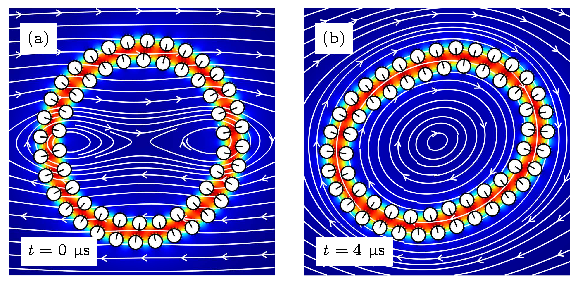
\includegraphics[width=11.5cm]{Figure3_Wrapper.pdf}
%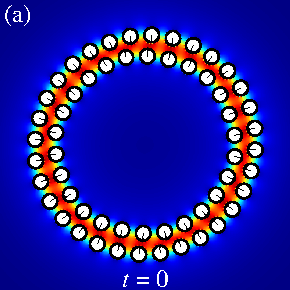
\includegraphics[width=0.3\textwidth]{N58_0.pdf}
%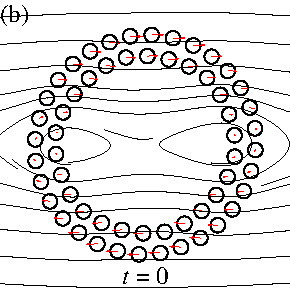
\includegraphics[width=0.3\textwidth]{N58_vel_0.pdf}\\
%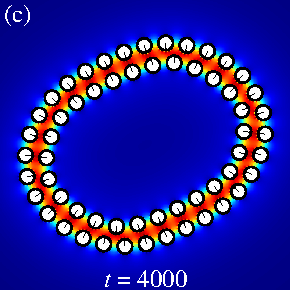
\includegraphics[width=0.3\textwidth]{N58_20000.pdf}
%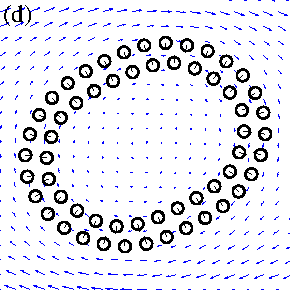
\includegraphics[width=0.3\textwidth]{N58_vel_20000.pdf}
  \caption{\label{figure3} 
  JP vesicles undergo tank-treading in shear flow. 
  In panel (a),  the initial, 58-body vesicle is circular and the black arrows point in the direction of the
  hydrophobic side of the JP.
  In panel (b), the JP suspension rotates and deforms with the shear flow.
  The color map is for the solution $u$ of \eqref{eq:SL}. 
  The white curves are the streamlines of $\uu.$ 
   The shear rate is $\chi=0.0025$.}
\end{figure}

\subsection{Model Parameters}
\cite{Fu20} studied physical quantities for static JP vesicles. 
In the present work, we study JP vesicles in various background flows.
We also perform parametric studies of effective properties of the JP vesicles 
as a function of particle size and interaction strength.
An analysis of the relationship between particle shape on effective properties is beyond 
the scope of the current paper. 

The particles are circular disks with centres 
$\aa_i$ and unit-length directors $\dd_i$ (Figure \ref{fig:figure0}(a)).
The simulations use the reference length $l_0 = 2.5$~nm representing the
thickness of a lipid monolayer.
The boundary conditions~\eqref{eq:SLbc} are $f_i(\xx) = \tfrac{1}{2}(1 + \cos
\theta_i)$ where $\theta_i$ is the angle between $\xx - \aa_i$ and
$\dd_i$.
We nondimensionalize the PDE systems 
\eqref{eq:stokes}-\eqref{eq:total_forces}
problem through the change of variables 
%\begin{equation}
%\label{eq:nondimensionalize}
$t \mapsto t \text{ ns}$,
$\xx \mapsto \xx \text{ nm}$, %\quad 
$\uu \mapsto \uu \text{ nm ns}^{-1}$, and %\quad 
$p \mapsto p \text{ pN nm}^{-2}$.
%\end{equation}
The numerical time step size is $\Delta t=0.2$.

The base-case is a single JP vesicle consisting of $N_b = 58$ particles
with $c = 0.5 l_0$ for particle radius, $\rho = 2 l_0$ for decay length, $\rho_0 = 0.2l_0$ for repulsion
length, $M=4.0$~$k_BT$ for repulsion strength, $\gamma = \text{4.1 pN
nm}^{-1}$ for interfacial tension.  The parameter $\mu = \text{1 cP} = \text{1 pN
ns nm}^{-2}$ is viscosity of room-temperature water. 

To reach consistent simulation outcomes, we first solve for a baseline
JP \ReviewerThree{vesicle} that is suitably close to equilibrium. We
start with an assumed configuration of $N=58$ JP in the form of two,
circular, apposing monolayers of about $8$ nm in radius. The norms of
the translational and rotational velocities vanish exponentially with an
approximate decay rate $\sim 4.6$ $\upmu$s$^{-1}$. An equilibrium
configuration is therefore rapidly attained. This equilibrium
configuration serves as the initial data in the subsequent background
flow simulations.

For a single JP vesicle, we consider background flows for a shear flow 
(Section \ref{sec:ves_in_shear}), 
a parabolic flow (Section \ref{sec:ves_in_parabolic}),
and a quiescent flow (Section \ref{sec:ves_in_parabolic}). 
In addition to observing the familiar tank-treading motion, the shear
flow studies yield a friction coefficient for inter-monolayer slip 
and a critical rupture shear rate.  Permeability coefficients and 
stretching moduli arise from analyzing stretched JP vesicles in the 
quiescent background flow case.  
 
%\subsection{Jeffery Orbit}
%We use Jeffery orbits to numerically validate our solver for the mobility-problem.  
%The background flow is a shear flow $\uu_{\infty}(\xx) = \dot\gamma  \xx \cdot \mathbf{e}_2 \mathbf{e}_1$ with shear rate $\dot\gamma$
%and orthogonal unit vectors $\mathbf{e}_1$ and $\mathbf{e}_2$. 
%A single elliptical particle is suspended in the fluid with centre at the origin.
%The Jeffrey orbit  
%\begin{equation}
%\label{eq:jeff}
%\Theta(t) = \tan^{-1}\left(\frac{a}{b}\tan \left(\frac{ab \dot\gamma t}{a^2+b^2}\right)\right)
%\end{equation}
%gives the angle between the major axis and $\mathbf{e}_2$
%where $a$, $b$ are the semi-major and semi-minor axes. 
%We are assuming $\Theta(0) = 0$.
%Figure~\ref{figure1} shows that the angles coming from the integral equation method \eqref{eq:SKIE}-\eqref{eq:mobility2}
%are in complete agreement with the theoretical time course \eqref{eq:jeff}.  Hydrophobic attraction and repulsion are zero for a single particle. 
%
%
%\begin{figure}
%\centering
%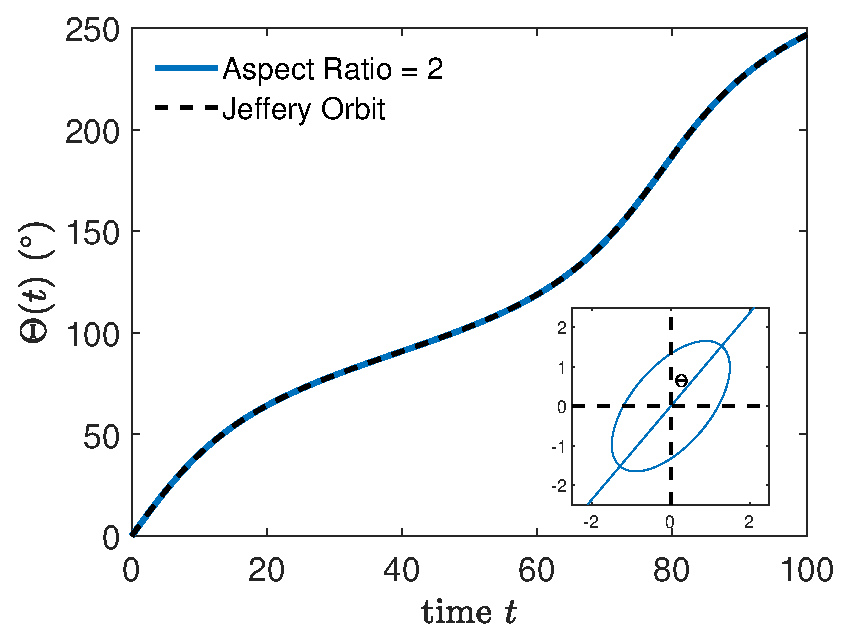
\includegraphics[width=0.4\textwidth]{JefferyOrbit2.eps}
%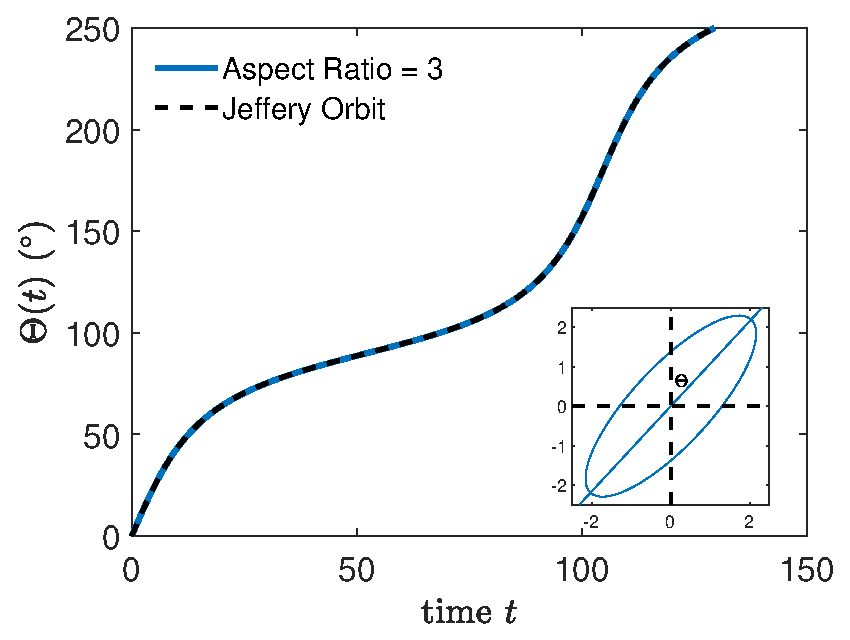
\includegraphics[width=0.4\textwidth]{JefferyOrbit3.eps}
%  \caption{The figure compares the theoretical Jeffery orbit for $\Theta(t)$ and the result from the integral equation method. 
%    The insets show the simulation setup. The shear rate is $\dot\gamma=0.1$.}
%    \label{figure1}
%\end{figure}

%%%%%%%%%%%%%%%%%%%%%%%%%%%%%%%%%%%%%%%%%%%%%%%%%%%%%%%%%%%%%%%%%%%%%%%



%%%%%%%%%%%%%%%%%%%%%%%%%%%%%%%%%%%%%%%%%%%%%%%%%%%%%%%%%%%%%%%%%%%%%%%

%\todo[inline]{Introduce dimensionless shear rate here (and check the numbers)}




%For the $N$-body Janus-vesicle, we denote a constant initial radius $R_0=\sqrt{A_0/4\pi}$ with initial area $A_0$

%referred from~\cite{Finken08} and~\cite{Shaqfeh11},
%\begin{align}
%  \chi = \dot\gamma \frac{\mu R_0^3}{\kappa},
%\end{align}
%%
%where $\dot\gamma$ the dimensional shear rate, and $\mu$ the fluid viscosity.


%%%%%%%%%%%%%%%%%%%%%%%%%%%%%%%%%%%%%%%%%%%%%%%%%%%%%%%%%%%%%%%%%%%%%%%
\subsection{Tank-Treading Vesicles}
\begin{figure}
\begin{center}
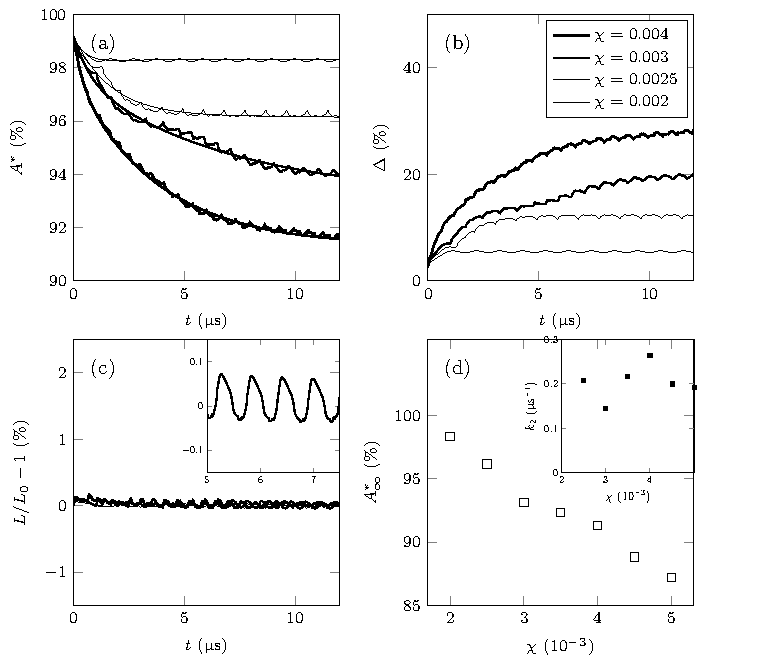
\includegraphics[width=13.5cm]{Figure4_Wrapper.pdf}
%\hspace{-0.6cm}
%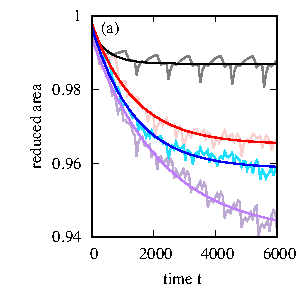
\includegraphics[height=2in]{ReducedArea.pdf}
%\hspace{0.6cm}
%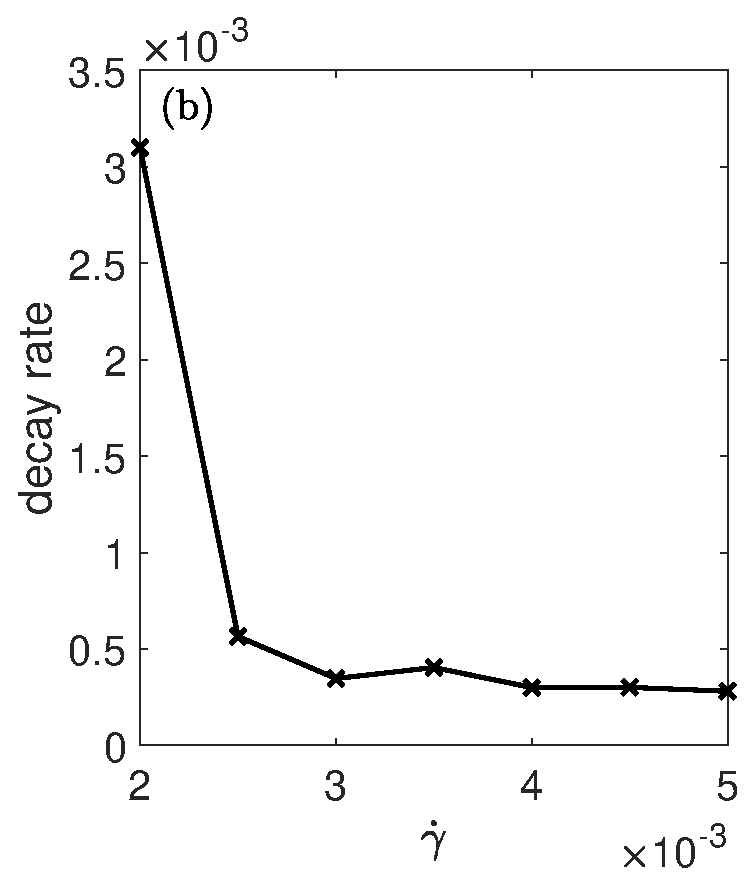
\includegraphics[height=2in]{DecayRate.eps}\\
%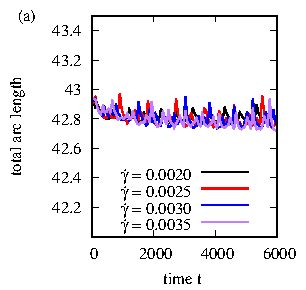
\includegraphics[height=2in]{ArcLength.pdf}
%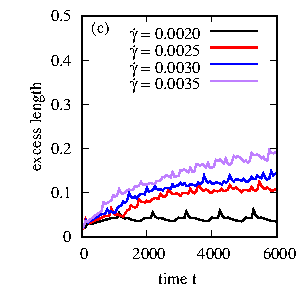
\includegraphics[height=2in]{ExcLength.pdf}
\end{center} 
  \caption{\label{figure4} JP vesicles lose enclosed area but conserve
  length in a shear flow. Panel (a) gives the reduced area over time for
  four different shear rates. The monotonic curves are a two-exponential
  best fit. There is a commensurate increase in excess length (panel
  (b)), but the arc length of the mid plane curve is more or less
  constant for all shear rates (panel (c)). The inset in panel (c) is
  for shear rate 0.003. The legend in panel (b) applies to panels
  (a)--(c). Panel (d) plots the steady-state reduced area and the decay
  rate $k_2$ (inset) coming from the fitting data in panel (a).}
\end{figure}

%%%%%%%%%%%%%%%%%%%%%%%%%%%%%%%%%%%%%%%%%%%%%%%%%%%%%%%%%%%%%%%%%%%%%%%
\subsubsection{Vesicle in a Shear Flow}
\label{sec:ves_in_shear}
Our simulation studies begin by showing, for the first time, that a JP
suspension with hydrophobic attraction behaves as a tank-treading
vesicle (\cite{Finken08, Shaqfeh11}). The centroid of the baseline,
$58$-body JP vesicle lies at the origin and the background shear flow 
\begin{align}
  \uu_{\infty}(\xx) = \dot\gamma (\xx \cdot \mathbf{e}_y) \mathbf{e}_x,
\end{align} 
is applied for shear rate $\dot\gamma$, and orthogonal unit vectors
$\mathbf{e}_x$ and $\mathbf{e}_y$ for the horizontal and vertical
directions, respectively. We use the dimensionless shear rate $\chi =
\dot \gamma$ (s$^{-1}$) ns.

\begin{figure}
\begin{center}
  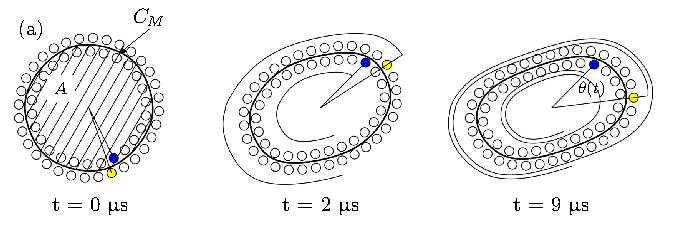
\includegraphics[width=11cm]{Figure5_Wrapper.pdf}\\
  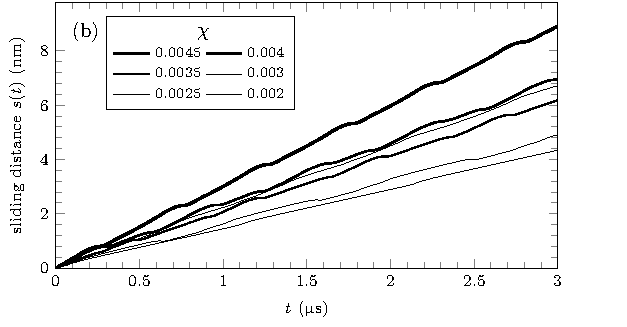
\includegraphics[width=11cm]{Figure5B_Wrapper.pdf}
%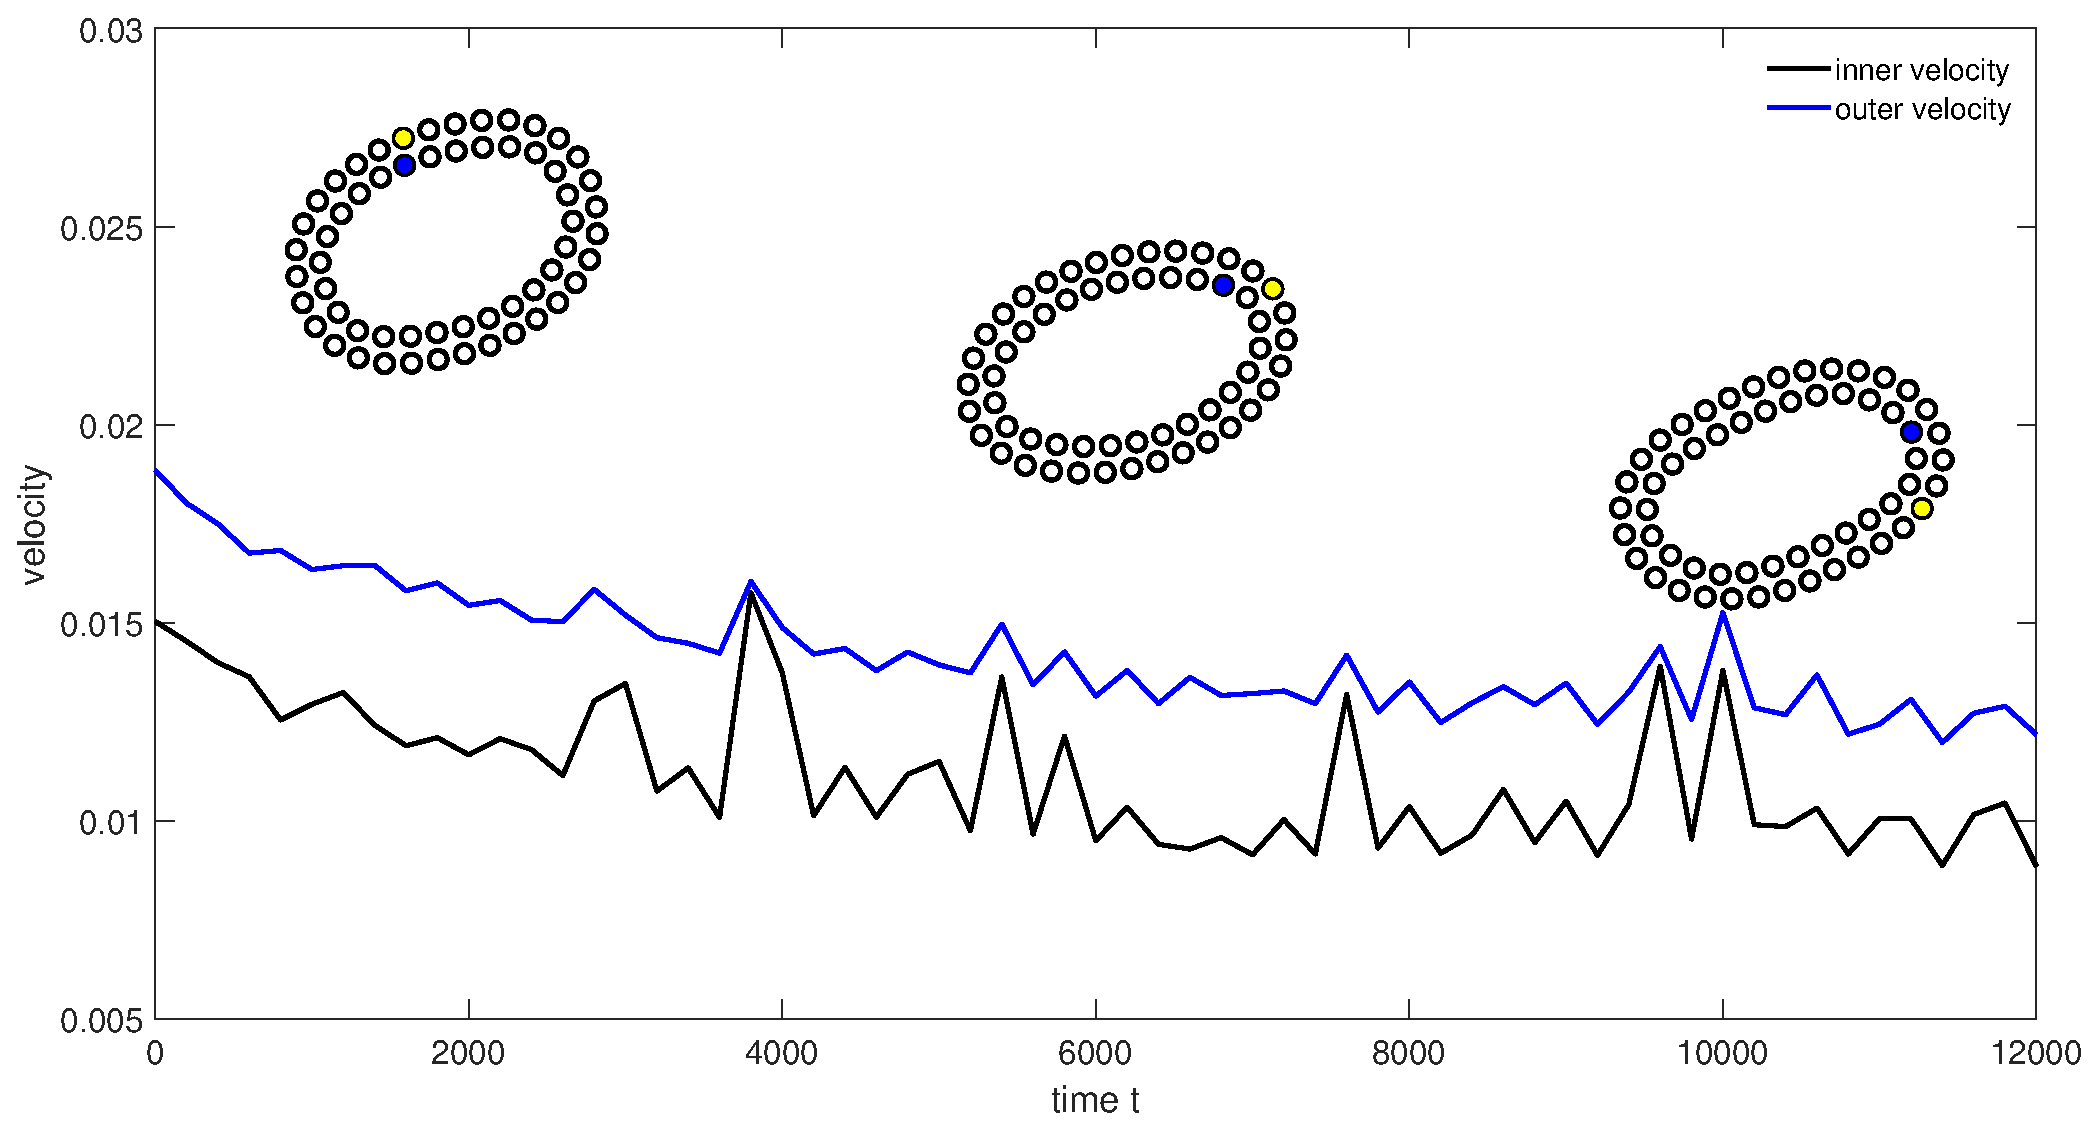
\includegraphics[width=0.5\textwidth]{Slip.eps}\\
%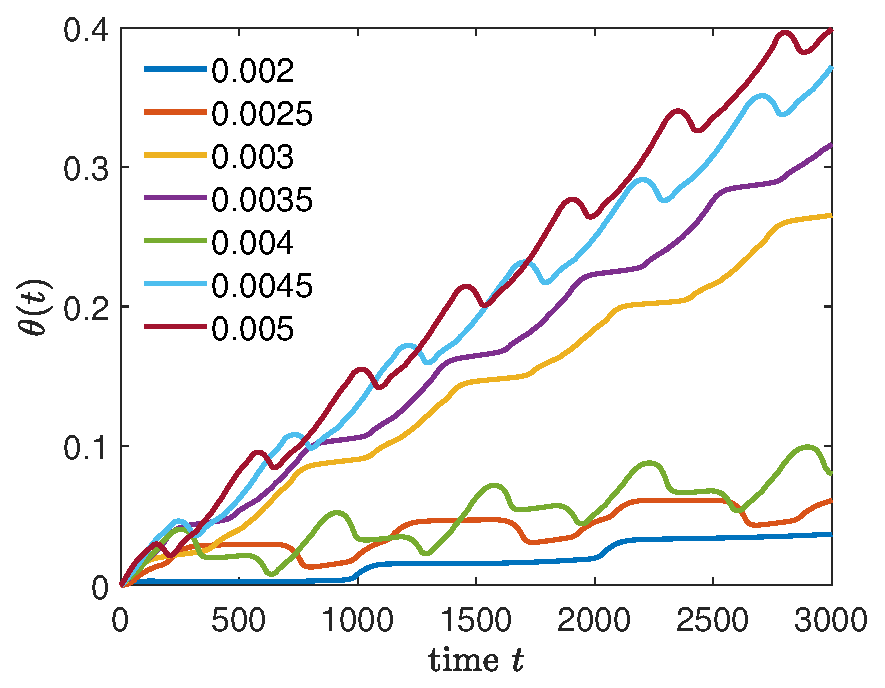
\includegraphics[width=0.4\textwidth]{Slip2.eps}
\end{center} 
\caption{\label{figure5} Inter-monolayer slip is present in the JP
  vesicle tank-treading motion at all shear rates. Panel (a) tracks a
  pair of particles (blue and yellow). The shear rate is $\chi=0.005$
  and in the right figure, the yellow particle will complete two and a
  quarter revolutions in the same time the blue particle completes two
  revolutions. The curves in panel (b) are the distance the outer
  leaflet has slid past the inner leaflet. The slopes of the curves
  give the slip velocity. With the exception of $\chi = 0.0035$, the
  slip velocity is generally monotonic in the shear rate.}
\end{figure}

Figure~\ref{figure3} shows snapshots of the JP vesicle in the shear flow
with $\chi=0.0025$. Under the background flow, the rigid-body boundary
condition~\eqref{eq:rigid_bc} causes the particle suspension to
elongate. This perturbation disrupts the preferred particle orientations
and exposes the hydrophobic core to bulk water (Figure~\ref{figure3},
red region). In response, hydrophobic
attraction~\eqref{eq:hydrophobicAttraction} causes the particles to
reorient and form a somewhat elliptically-shaped suspension. Panel (a)
shows the initial configuration and panel (b) shows the later,
fully-formed, clockwise tank-treading motion. The JP suspension
maintains its bilayer structure throughout the simulation. 
%

To extract physical quantities, let $A^* = 4\pi A/L^2$ be the reduced
area and $\Delta=L/\sqrt{A/\pi} - 2\pi$ the excess length of the bilayer
structure (\cite{Finken08}). Here, $A$ is the enclosed area and $L$ is
the total length of the JP vesicle (Figure \ref{fig:figure0}a).
Figure~\ref{figure4} shows the evolution of the area and length for
various shear rates. Panels (a) and (b) show that $A^*$ decreases and
$\Delta$ increases with time, respectively, and that the rate of
decrease/increase grows with shear rate. The total arc length, however,
remains constant for all time for all four shear rates (panel (c)). We
conclude that the JP vesicle loses area and that the bilayer behaves as
a permeable membrane. 

Since the starting configuration is nearly circular, the reduced area
decreases from an initial value close to $1$ and tends to a steady-state
value $A^*_{\infty}$. The data in panel (a) are fit to the model $A^* =
(A^*_{\infty}-a_1-a_2) + a_1 \exp(-k_1t) + a_2 \exp(-k_2t),$ $0 < k_2 <
k_1$. Panel (d) shows that $A^*_{\infty}$ decreases with the shear rate.
The JP vesicle achieves a steady-state reduced area earlier when the
shear rate is low (inset), but the decay rate $k_2$ is more or less
constant for higher shearer rates. 

The oscillations in the data of Figure~\ref{figure4} are due to the
granularity of the JP vesicle. The inset of Figure~\ref{figure4}c zooms
in on the arc length data for the shear rate $\chi = 0.003$. It shows
that the oscillations are smooth and well-resolved by our second-order
Adams-Bashforth scheme.

We point out that the range of values for $\chi$ where we measured for
tank-treading correspond to shear rates $\dot \gamma = \mathcal{O}(10^6$
s$^{-1}$) which gives fluid velocities $\mathcal{O}($m s$^{-1}$$)$ in
the vicinity of the vesicle. While large, these orders of magnitude are identical to
ones used in prior MD studies (\cite{Brandner2019}) and are a
consequence of the fact that larger shear rates are required to produce
the viscous stresses needed to appreciably deform smaller vesicles. 

%%%%%%%%%%%%%%%%%%%%%%%%%%%%%%%%%%%%%%%%%%%%%%%%%%%%%%%%%%%%%%%%%%%%%%%
\subsubsection{Inter-Monolayer Friction}
We observe inter-monolayer slip in the tank-treading, JP vesicle at all
shear rates. Since they are not bound, the two leaflets of the vesicle
are able to slide past one another. 
Monolayer slip effects have been incorporated in continuum models (\cite{sch-vla-mik2010}).
In the present setting, slip is limited by viscous
friction of the aqueous gaps between particles and by the constant
unbinding and binding of particles pairs in apposing leaflets. 


Figure~\ref{figure5}a illustrates inter-monolayer slip by tracking the distances
traveled by a pair of particles along the midplane curve. In the left image, the blue and yellow
particle lie next to each other. In the right-most panel, the yellow
particle has traveled farther than the blue particle. This suggests that
the outer tangential velocity, obtained by projecting the velocity of the
outer leaflet onto the midplane curve, 
is larger than that of the inner leaflet. 

From the data, we obtain an inter-monolayer friction coefficient 
\begin{align}
  b =  \frac{\langle F \rangle}{\langle L   U \rangle} ,
\end{align}
where $F$ is the tangential force jump, $L$ is the length of the
midplane $C_M$ (Figure~\ref{figure5}a), and $U$ is the slip velocity.
The time average $\langle \cdot \rangle$ is necessary to avoid division by zero
whenever slip velocity vanishes.  

%original table
%\begin{table}
%\caption{Friction Coefficients}
%\centering
%\begin{tabular}{c c c c c c c c }
% $\dot\gamma$  (ns$^{-1}$) & 0.0020   &  0.0025 &  0.0030 &  0.0035 &  0.0040 & 0.0045 & 0.0050  \\
%\hline                    
%$b$ (pN ns nm$^{-3}$)    & 0.43 & 1.19 &   0.42  & 0.69 &   0.97  &   0.80  &  1.07 \\ 
%\hline    
%\end{tabular} 
%\label{table1}
%\end{table}

%updated table
\begin{table}
\caption{Friction Coefficients $b$ (pN ns nm$^{-3}$) \\
}
\centering
\begin{tabular}{c c c c c c c c c }
& & & & $\dot\gamma$  (ns$^{-1}$) & & & &\\
\cline{2-8}\\
 & 0.0020   &  0.0025 &  0.0030 &  0.0035 &  0.0040 & 0.0045 & 0.0050  & Average\\
\cline{1-8}\\
$N_b=53$  & 0.50  & 0.51  &  0.44 & 0.52  & 0.45 &  0.57   &  0.62 & 0.52  \\ 
$N_b=56$ & 0.54 & 0.41 & 0.35  & 0.37 & 0.43 & 0.76  & 0.70 & 0.51\\ 
$N_b=58$   & 0.42 & 0.63 & 0.50   & 0.40  & 0.48  & 0.53 & 0.55 & 0.50 \\   % new
$N_b=61$  & 0.22 & 0.36 & 0.41   & 0.45  & 0.45 & 0.44   & 0.44 & 0.40\\ 
\end{tabular} 
\label{table1}
\end{table}


The tangential force jump $F$ equals the 
tangential shear force on the outer
leaflet minus the tangential shear force on the inner leaflet. 
To calculate  $F$, we first let 
\begin{align}
F_h = \int_{\mathcal{C}_M^+} 
  \ttau \cdot \sigma \cdot \nnu \,\dif s - \int_{\mathcal{C}_M^-} 
 \ttau \cdot \sigma \cdot \nnu \,\dif s 
\end{align}
where $C_M^+$ and $C_M^-$ are target curves obtained by projecting the
midplane curve $C_M$  a distance $h$ outward,
respectively inward, along its unit normal vector field (Figure~\ref{figure5}a). We sample $F_h$ for 
$h = \pm 1.3, \pm 1.5,  \pm 1.7, \pm 1.9$ times the particle radius and define $F$ by
extrapolating to zero distance. This avoids integrating along a curve passing directly through the
particles.   

To calculate $U$, we let $u_+(\mathbf{x})$ and $u_-(\mathbf{x})$ 
be the tangential velocity of the outer, respectively inner, leaflet.  Then 
\begin{equation}
  U = \frac{1}{L}\int_{C_M}\left(u_+(\mathbf{x})(1 - \delta \kappa) -
  u_-(\mathbf{x})(1 +  \delta \kappa)\right) \, ds,
\end{equation}
where $ \delta $ is the distance from the leaflet centres to the midplane and $\kappa$ is the curvature. 
The factors $\pm  \delta \kappa$ are needed to project the leaflet velocities, defined on the particle centres,
onto the midplane curve. 
Finally, the function $s(t) = \int_0^t dU $ records the distance one leaflet has
slid past the other. Figure~\ref{figure5}b plots the sliding distance for various shear
rates. 

%Table~\ref{table1} provides $b = 0.79 \pm 0.3$ pN ns nm$^{-3}$  
\ReviewerOne{Table~\ref{table1} provides a series of numerical friction coefficients $b$ and the default number of particles is $N_b = 58$. With the fixed total length of the JP vesicle, we change parameters related to the length scale, for instances, $\rho$, $\rho_0$, and the radius of particles.
With $-5\%$, $5\%$, and $10\%$ adjustments in these parameters, the resulting numbers of particles are $N_b=\{61,56,53\}$, respectively. }
%
\ReviewerOne{There is no clear trend shown in Table~\ref{table1} but these values of $b$ are}
%over a range of shear rates which is 
in good quantitative agreement with values previously reported in the literature.
Atomistic studies have also considered inter-monolayer slip in lipid bilayers. 
\cite{WuoEd06} and \cite{denOtter2007} reported $b = 0.7 \times 10^6$ Pa m$^{-1}$ s  
$=0.7$ pN ns nm$^{-3}$  
and $b = 2.4$  pN ns nm$^{-3}$ for DPPC membranes simulated by MD, respectively. 
Using a more recent version of the Martini force field, \cite{Zgorski2019} 
gives $b = 5.5$ pN ns nm$^{-3}$ for shear rates 0.4 ns$^{-1}$ and higher.
It is understandable that there is uncertainty in the friction coefficients of
Table~\ref{table1}.  The scatter in our data, however, is fully consistent with that calculated
from MD simulations, c.f. the transient rise in values of Table~\ref{table1} and in \cite{Zgorski2019}, Figure 10
for low shear rates. 
\subsubsection{Membrane Ruptures}
\begin{figure}
\centering
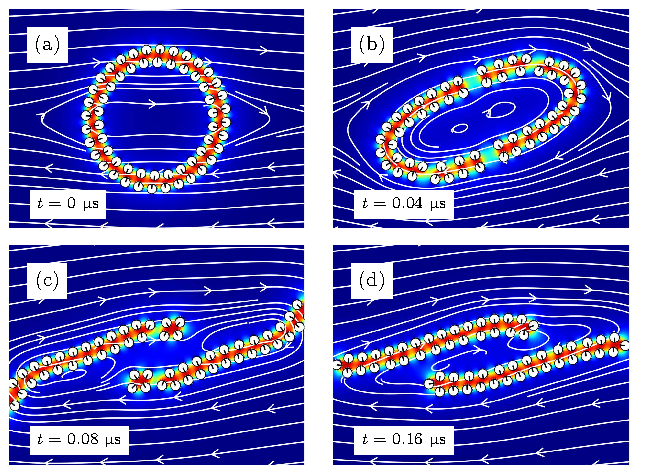
\includegraphics[width=11.32cm]{Figure8_Wrapper.pdf}
%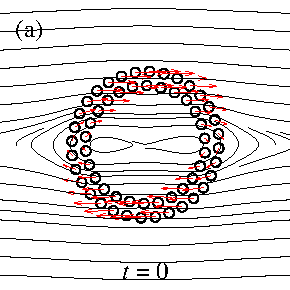
\includegraphics[height=2in]{N58_rupt_0.pdf}
%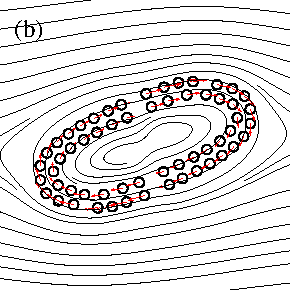
\includegraphics[height=2in]{N58_rupt_200.pdf}
\\
%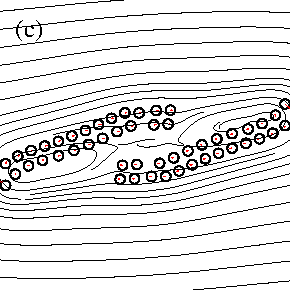
\includegraphics[height=2in]{N58_rupt_400.pdf}
%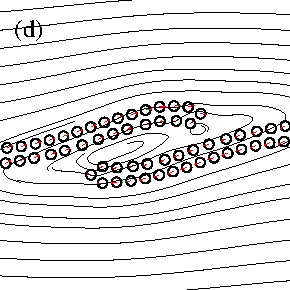
\includegraphics[height=2in]{N58_rupt_600.pdf}
  \caption{\label{figure8} Tank-treading leads to membrane rupture for
  large shear rates.} 
\end{figure}
A temporary fissure or a complete membrane rupture can occur at large
shear rates. Figure~\ref{figure8} demonstrates how a vesicle can rupture
when suspended in a shear flow. For $\chi = 0.1$, starting with a
circular shape (Figure~\ref{figure8}a), the vesicle is stretched by the
background flow and fissures appear in the bilayer structure in multiple
locations (Figure~\ref{figure8}b). In Figure~\ref{figure8}c, the
ruptured vesicles form two planar micelles which are eventually carried
off by the flow (Figure~\ref{figure8}d). 
%
\ReviewerOne{An emperical numerical study has shown that the critical shear rate for a complete membrane rupture is $\chi=0.0655$. Supplementary Materials Movie 4 shows the membrane rupture at the critical shear rate.}




%%%%%%%%%%%%%%%%%%%%%%%%%%%%%%%%%%%%%%%%%%%%%%%%%%%%%%%%%%%%%%%%%%%%%%%
\subsubsection{Vesicle in a Parabolic Flow}
\label{sec:ves_in_parabolic}
Finally, we consider the parabolic background flow
\begin{align}
  \uu_\infty = v_{max}\left[ 1 - \left( 
    \frac{\xx \cdot \mathbf{e}_y}{wR_0}\right)^2
    \right]\mathbf{e}_x,
\end{align}
%
where $v_{max}$ is the flow strength and $w$ determines the shape of the
flow. The parameter $R_0$ is the radius of the JP vesicle at $t=0$ and
$w$ sets the width of the profile. \cite{Kaoui09, cou-kao-pod-mis2008,
dan-vla-mis2009} have shown that the behaviour of a vesicle in this
unbounded flow includes vertical migration, and depending on the flow
rate and reduced area, the steady-state shape can be either a symmetric
parachute or an asymmetric slipper.

%Besides the tests of a JP vesicle in a shear flow, an interesting
%test can also use the proposed model and the setup. Consider a
%symmetric parabolic flow about the $x$-axis,~\cite{Kaoui09} studied
%shapes of the red blood cell immersed in a parabolic flow using a
%continuum model. With a similar setup, the background flow for this set
%of simulations is given by

Figure~\ref{figure6} shows four configurations for one specific case
where the centroid of the JP vesicle is initially placed slightly above
the $x$-axis. We have marked a pair of particles blue and yellow in the
inner and outer leaflets, respectively, and observe that the deformed JP
vesicle (Figure~\ref{figure6}, $t = 12~\upmu$s) has a counterclockwise
movement and the shape of the vesicle approaches an asymmetric slipper
shape. For this test, the reduced area in the final configuration is
approximately $0.9$ which matches the previous numerical tests
in~\cite{Kaoui09} where a slipper-like shape occurs when the flow
velocity is weak and the reduced area is large. The flow causes the
vesicle, which is initially placed above the axis, to drift downward
where it reaches a steady height of about $1$ nm. 

\begin{figure}
\centering
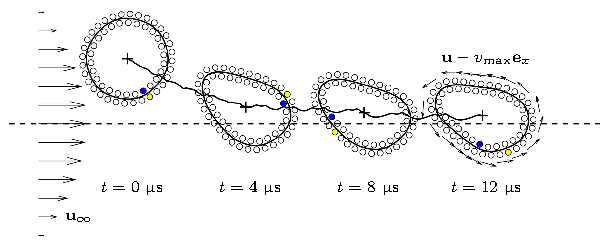
\includegraphics[width=\textwidth]{Figure6_Wrapper.pdf}
%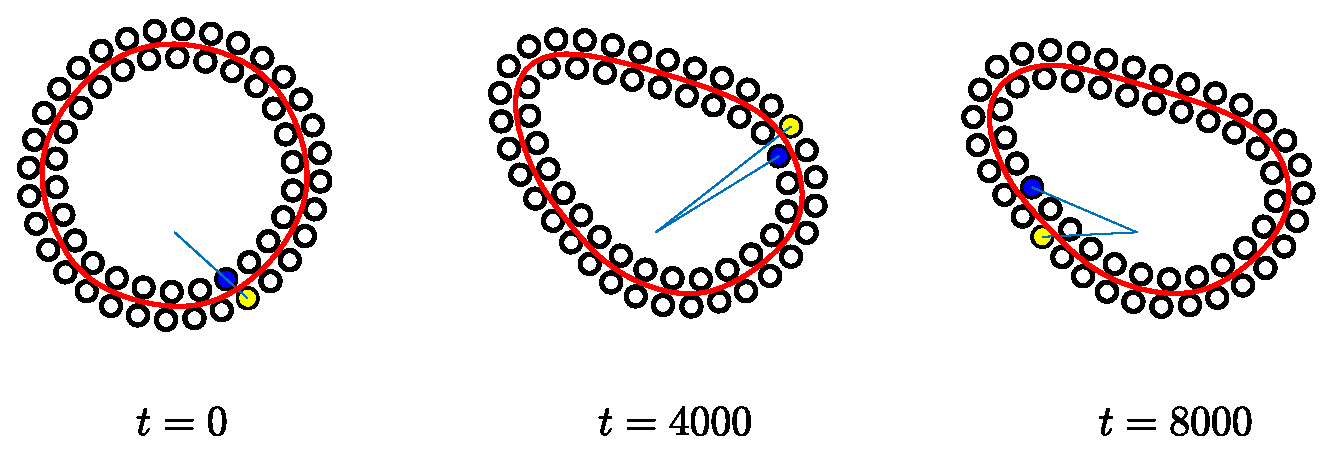
\includegraphics[width=0.8\textwidth]{slipper.eps}
  \caption{\label{figure6} A JP vesicle placed in a parabolic flow
  drifts toward the central axis. It assumes a slipper shape and
  undergoes tank-treading motion like in the shear flow case. The arrows
  on the left illustrate the background flow and the arrows on the right
  show the velocity relative to the vesicle's moving frame. The thick
  black curve plots the distance from the axis as a function of time
  from left to right. The parameters are $v_{max} = 8$~nm ns$^{-1}$,
  $w=10$, and $R_0=20$ nm.}
\end{figure}


%%%%%%%%%%%%%%%%%%%%%%%%%%%%%%%%%%%%%%%%%%%%%%%%%%%%%%%%%%%%%%%%%%%%%%%


\subsection{Stretching and Permeability}
\label{sec:ves_in_quiescent}
\begin{figure}
\centering
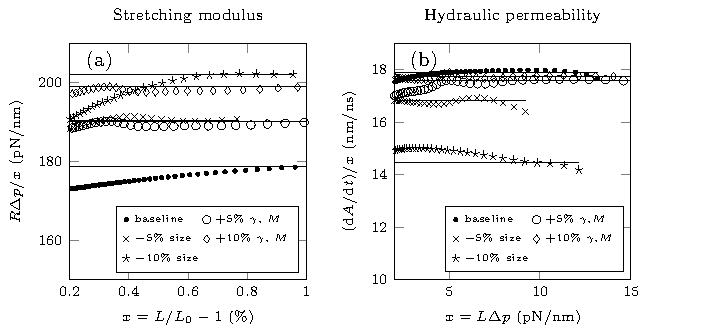
\includegraphics[width=\textwidth]{Figure2_Wrapper.pdf}
%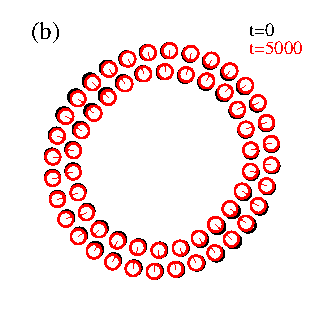
\includegraphics[height=2in]{relax2.eps}
%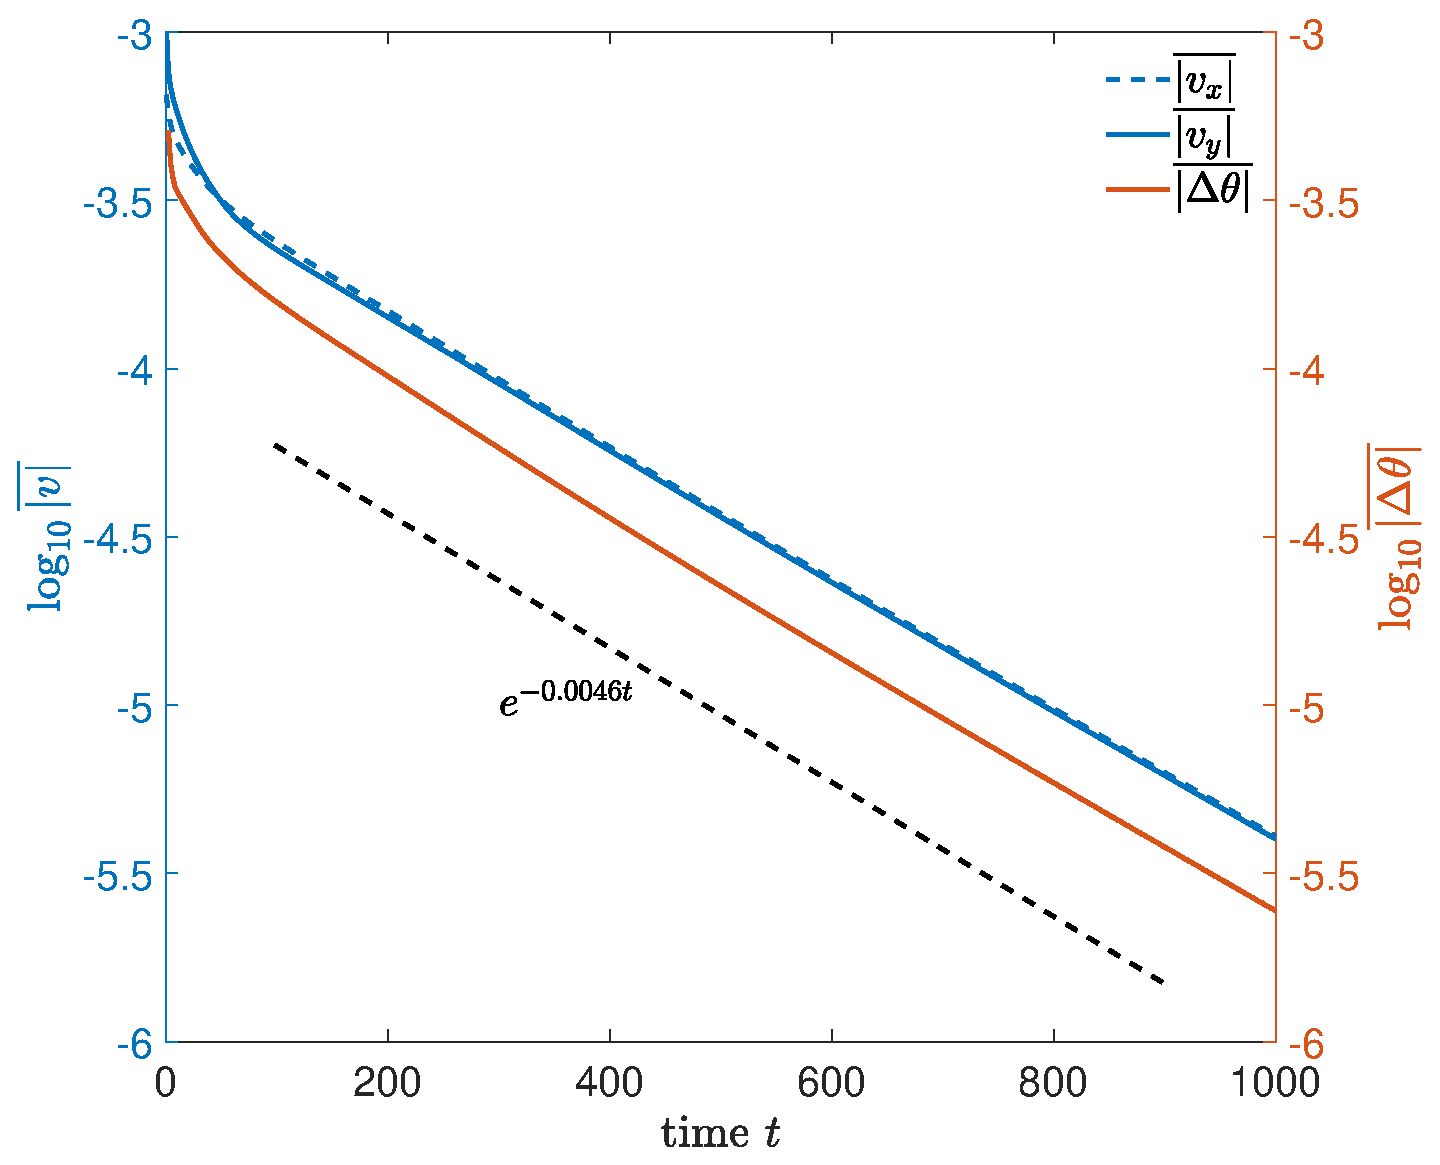
\includegraphics[height=2in]{relax.eps}\\
%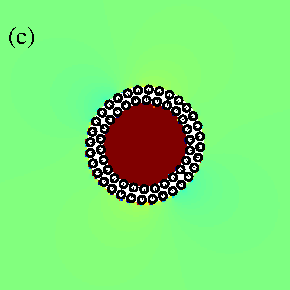
\includegraphics[height=2.in]{N58_0pres.pdf}
%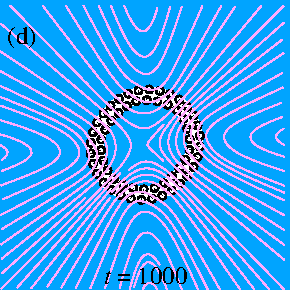
\includegraphics[height=2.in]{N58_5000pres.pdf}
%  \todo[inline]{Put pressure of each of the two configurations below
%  this.}
\caption{\label{figure2} In JP vesicles, tension and pressure relax as
  fluid is expelled through the particle interstices. In panel (a), the
  thin curve plots the mean of the norm of the particle translational
  velocities. The thick curve plots the mean of the absolute value of
  the particle angular velocities. At $t = 0$ $\upmu$s, the vesicle has
  a spatially constant internal pressure 0.05~pN nm$^{-2}$ (red color,
  panel (b)). In panel (c), pressure has dissipated and the vesicle has
  moved from its initial configuration (gray circles), to the
  equilibrium configuration (black circles). The data in panels (d) and
  (e) support the linear relationship expressed by
  \eqref{eq:LaplacePressure} and \eqref{eq:perm}. Circles are for a
  vesicle with 17 nm initial radius; square are for a 34 nm initial
  radius. Asterisks are for a 18 nm initial radius but with smaller,
  1.25 nm diameter particles. In panel (f), the theoretical time course
  \eqref{eq:perm_solution} overlaps the data using constants $K_A$ and
  $P$ derived from panels (d) and (e). }
\end{figure}
Finally, we show that the JP vesicle behaves as a permeable membrane and the inextensibility comes
about due to a large stretching modulus.
%an extensible, permeable membrane. 
Figures~\ref{figure2}b shows an initial, non-equilibrium JP
vesicle suspended in a quiescent flow $\uu_{\infty} = 0$. The color map
plots the pressure $p$. The red color in Figures~\ref{figure2}b shows a
spatially constant, positive internal pressure (0.05~pN nm$^{-2}$) and the white
shows a spatially constant zero, external pressure. There is some fluid flow and
the pressure vanishes as the configuration tends toward the equilibrium
state (Figures~\ref{figure2}c).

What could be the source of this drop in pressure? In membrane
continuum  mechanics, small changes in surface area give rise to a membrane tension
$\tilde \gamma = K_A(A/A_0 - 1)$ where $A$ is the membrane surface area
and $A_0$ is the reference surface area. The area modulus $K_A$ of
bilayers is about $240$ pN nm$^{-1}$ (\cite{NaTr00}). In the
two-dimensional vesicles, the tension becomes
\begin{align}
\label{eq:stretch}
\tilde \gamma = K_A\left(\frac{L}{L_0} - 1 \right),
\end{align}
where $L$ and $L_0$ are the vesicle arc length and resting length,
respectively. Moreover, stretched, circular vesicles \ReviewerOne{have}
a Laplace pressure 
\begin{align}
\label{eq:LaplacePressure}
\Delta p = \frac{\tilde \gamma}{R},
\end{align}
where $\Delta p$ is the difference in internal pressure to the pressure
at infinity and $R^{-1}$ is the total curvature of the circular
cylinder.



Figure~\ref{figure2}c plots the data for the pressure jump $\Delta p$
between the particle centre and the far-field (see
Figures~\ref{figure2}c and~\ref{figure2}d). We use $R = L/(2\pi)$ for
the vesicle radius, and the horizontal axis is the relative stretch.
The circles are data for a vesicle with radius 17 nm. The linear fit
(solid lines) shows that $R\Delta P$ is proportional to the relative
stretching $L/L_0 - 1$. The squares are for a vesicle with twice the
radius 34 nm, and the data overlap supports that the proportionality
constant $K_A$ is a stretching modulus that is independent of vesicle
size. The data give $K_A = 170 \pm 9$ pN nm$^{-1}$ which is in good
agreement with the experimentally obtained area moduli of lipid bilayer. 
%
The reason the tank-treading vesicle appears inextensible ($L$ is more or less constant in Figure~\ref{figure4}c) is because the modulus $K_A$ is large.
%
To evaluate how changes to particle size lead to different
physical properties, the asterisk symbols are for an 18 nm radius
vesicle consisting of particles with diameter 1.25 nm, instead of the
usual 2.5 nm. These data give a smaller stretching modulus of $K_A =
102$~pN~nm$^{-1}$. 

The particles in our setup do not abut but rather have small gaps due to
repulsive forces. The gaps allow for some fluid flux across the JP
bilayer, and in membrane mechanics aqueous flux is quantified by the equation
\begin{align}
  \label{eq:perm} 
  \frac{dA}{dt} = -P L \Delta p,
\end{align}
where $P$ is a hydraulic permeability constant (\cite{chabanon2017,
qua-gan-you2021}). Figure~\ref{figure2}e shows that the data for
$L\Delta p$ and $dA/dt$ obey the linear relationship expressed by
\eqref{eq:perm}. The slopes of the linear fits give the hydraulic
permeabilities $P = 0.0296$ nm$^3$ ns$^{-1}$ pN$^{-1}$ and $P = 0.0283$
nm$^3$ ns$^{-1}$ pN$^{-1}$ for the 17 nm and 34 nm radius cases,
respectively. Like the area modulus, the data give a permeability 
that is independent of vesicle size.

\begin{figure}
\begin{center}
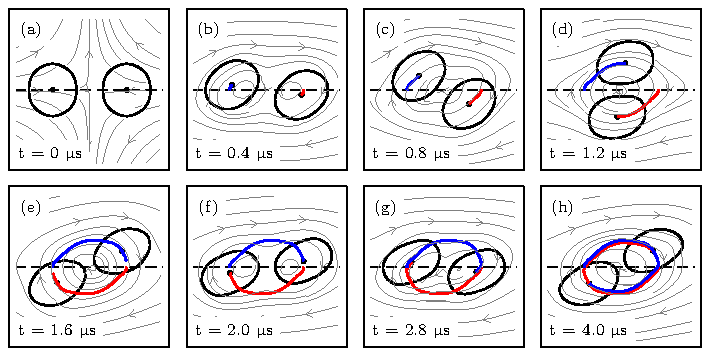
\includegraphics[width=\textwidth]{Figure9_Wrapper.pdf}
%  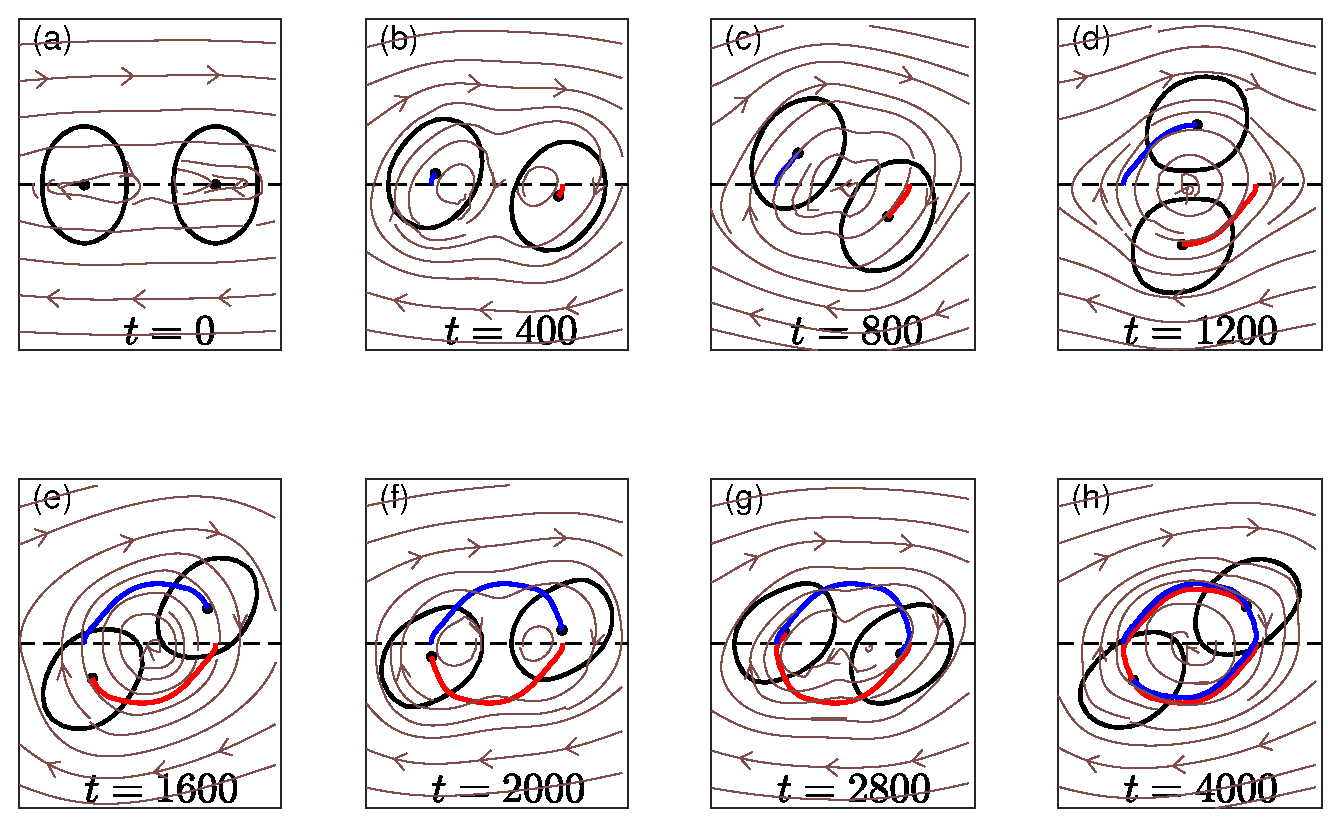
\includegraphics[width=0.9\textwidth]{ShearTraj.eps}
\end{center} 
  \caption{\label{figure9} Two JP vesicles suspended in a shear flow
  interact by orbiting about the origin. The moving paths of the two
  centroids are plotted in blue and red. The centroids are initially
  located on the $x$-axis. The fluid velocity streamlines appear in
  grey.  The dimensionless shear rate is $\chi=0.005$.}
\end{figure}

The hydraulic permeability we calculate, however, is not in agreement
with experimentally derived values and is larger by a few orders of
magnitude. We suspect this discrepancy is due to inter-particle distance
of the JP being large compared to the inter-lipid spacing in real
bilayers. To test this, we calculate the permeability for the particles
with diameter 1.25 nm. Due to their smaller size but fixed repulsion
strength, these particles have a larger inter-particle spacing resulting
in an increase in permeability, $P = 0.0566$~nm$^3$~ns$^{-1}$~pN$^{-1}$
(Figure~\ref{figure2}e, asterisk symbols).

Since the vesicles in Figure~\ref{figure2}a are nearly circular, we can
combine~\eqref{eq:stretch},~\eqref{eq:LaplacePressure},
and~\eqref{eq:perm}, to derive
\begin{align}
\label{eq:perm_solution}
L_0(L-L(0)) + L_0^2 \ln\left|\frac{L-L_0}{L(0)-L_0}\right| = -4\pi^2 P K_A t.
\end{align}
All in all, the theoretical time courses for \eqref{eq:perm_solution} are in good
quantitative agreement with the JP data (Figure~\ref{figure2}f).


% table 2


\begin{table}
\caption{Stretching Moduli and Permeabilities}
\centering
\begin{tabular}{ c c c c c c c }
 radius ($l_0$) &  $\rho$ ($l_0$)  &  $\rho_0$ ($l_0$) &  $M (k_BT)$ & $\gamma$ (pN nm$^{-1})$ & $K_A$ (pN nm$^{-1}$) & $P$ (nm$^3$ ns$^{-1}$pN$^{-1}$) \\
\hline      \hline 
 0.5 & 2.0  &   0.5  & 4.0 &  4.1  & 170$\pm9$   &  0.0296\\ 
%
 0.475 & 1.9  &   0.475  & 4.0 &  4.1   & 184$\pm5$  &  0.0283 \\ 
%
 0.45 & 1.8  &   0.45  & 4.0   &  4.1   & 189$\pm6$  &  0.0252  \\ 
%
 0.5 & 2.0  &   0.5  & 4.2   &  4.31  & 185$\pm5$  &  0.0292  \\ 
%
 0.5 & 2.0  &   0.5  & 4.4   &  4.51  & 195$\pm5$  &  0.0294 \\ 
\end{tabular} 
\label{table2}
\end{table}
%

\ReviewerOne{Table~\ref{table2} provides the results of stretching moduli $K_A$ and permeabilities $P$ for various cases. The default setup is shown in the first row. The next two rows show the results for the cases where the length scale related parameters are decreased by 5$\%$ and 10$\%$. One can observe that the constant $K_A$ increases 
and $P$ decreases as size of particles decreases. 
The last two rows demonstrate the results when the force related parameters $\gamma$ and $M$ are adjusted by 5$\%$ and 10$\%$. The quantities examined for these two cases show that $K_A$ increases and $P$ remains constant as inter-particle interaction strength increases. As expected by the fact that the permeability is dependent of the particle size where the gap between each adjacent JP pair is controlled by the size of JP. However, the detailed correlation between all model parameters will be explored as 
a direction of future work.}

%%%%%%%%%%%%%%%%%%%%%%%%%%%%%%%%%%%%%%%%%%%%%%%%%%%%%%%%%%%%%%%%%%%%%%%
\subsection{Two Vesicles in a Linear Flow}



\begin{figure}
  \centering
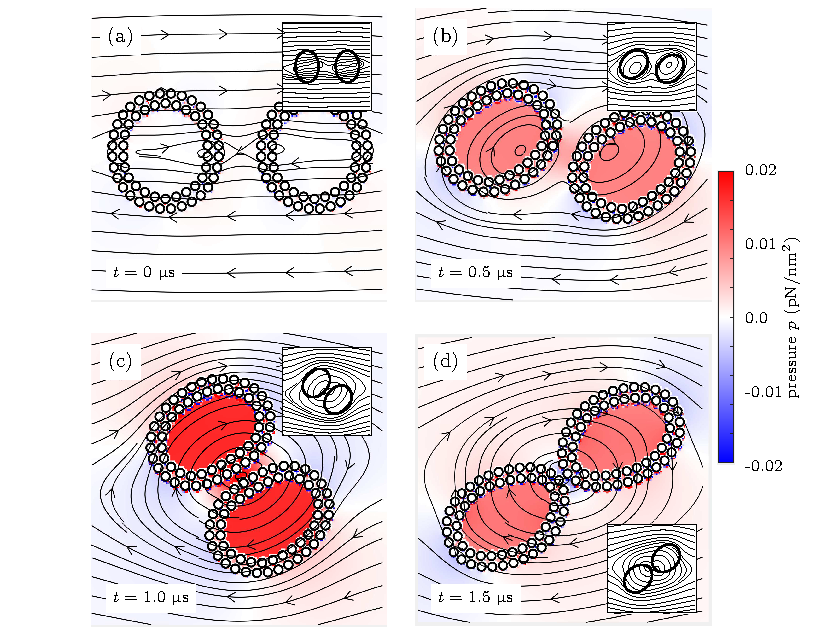
\includegraphics[width=\textwidth]{Figure10_Wrapper.pdf}  
%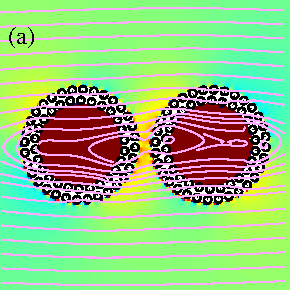
\includegraphics[height=2in]{N116_shear_0.pdf}
%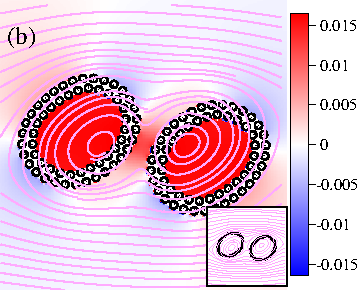
\includegraphics[height=2in]{N116_shear_2500.pdf}\\
%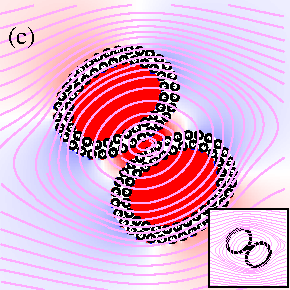
\includegraphics[height=2in]{N116_shear_5000.pdf}
%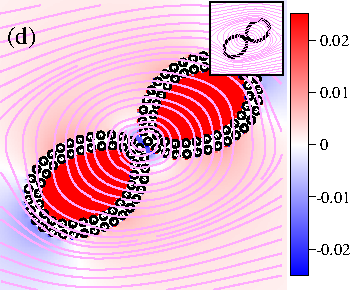
\includegraphics[height=2in]{N116_shear_7500.pdf}
  \caption{\label{figure10} 
  The figure is for the same simulation as in Figure~\ref{figure9}, 
  but also plots the fluid pressure $p$. The color bar is identical for all panels. 
  Internal pressure is initially zero, but then grows as the vesicles come close to contact  (panel (c)).
  The insets are generated from simulations of a continuum model of the vesicles (\cite{qua-vee-you2019}). 
  The streamlines of the two models are in agreement.}
\end{figure}

%%%%%%%%%%%%%%%%%%%%%%%%%%%%%%%%%%%%%%%%%%%%%%%%%%%%%%%%%%%%%%%%%%%%%%%
\subsubsection{Shear Flow}
Finally, we can study vesicle-vesicle interactions in background flows. 
Figure~\ref{figure9} shows the simulation of two JP vesicles suspended
in a shear flow with shear rate $\chi=0.005$. We duplicate the
pre-relaxed $58$-body JP vesicle from previous sections and construct the
initial configuration shown in Figure~\ref{figure9}a. The two centroids
are at coordinates $(-25,0)$ and $(25,0)$ in nm. In all panels, the blue and red
curves show the trajectory of the two JP vesicle centroids. They have
nearly completed a full period by $t=4$ $\upmu$s. 

We show snapshots of the fluid pressure in Figure~\ref{figure10}. Since the
initial JP vesicles are pre-relaxed, there is initially no pressure jump
between the internal and external fluids (panel (a)). Panels (b)--(d)
show the configurations when $t = \{0.5,1,1.5\}$ $\upmu$s, and the
streamlines are plotted in the background for all panels. 
We include the numerical results from a continuum model in all insets and these
comparisons give a qualitative agreement between two models.
We also observe an adhesive
effect between the two JP vesicles that is set up by the hydrophobic
attraction (Figure~\ref{figure10}c). Similar dynamics have been observed between a pair of adhering vesicles in a shear flow
(\cite{qua-vee-you2019, abb-far-ezz-ben-mis2021}). This adhesive
behaviour is absent when two JP vesicles are well-separated.

\begin{figure}
\begin{center}
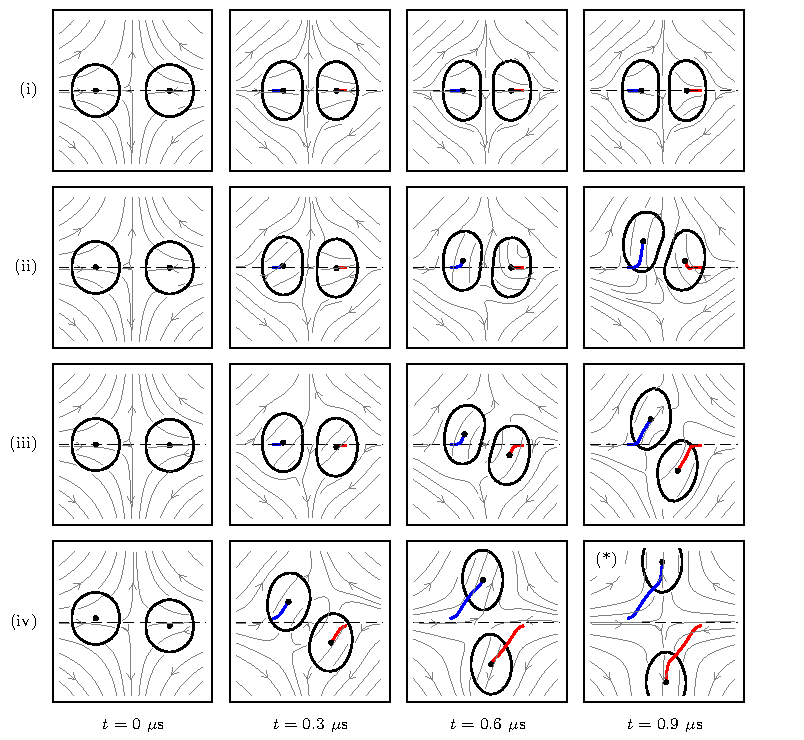
\includegraphics[width=0.97\textwidth]{Figure11_Wrapper.pdf}
%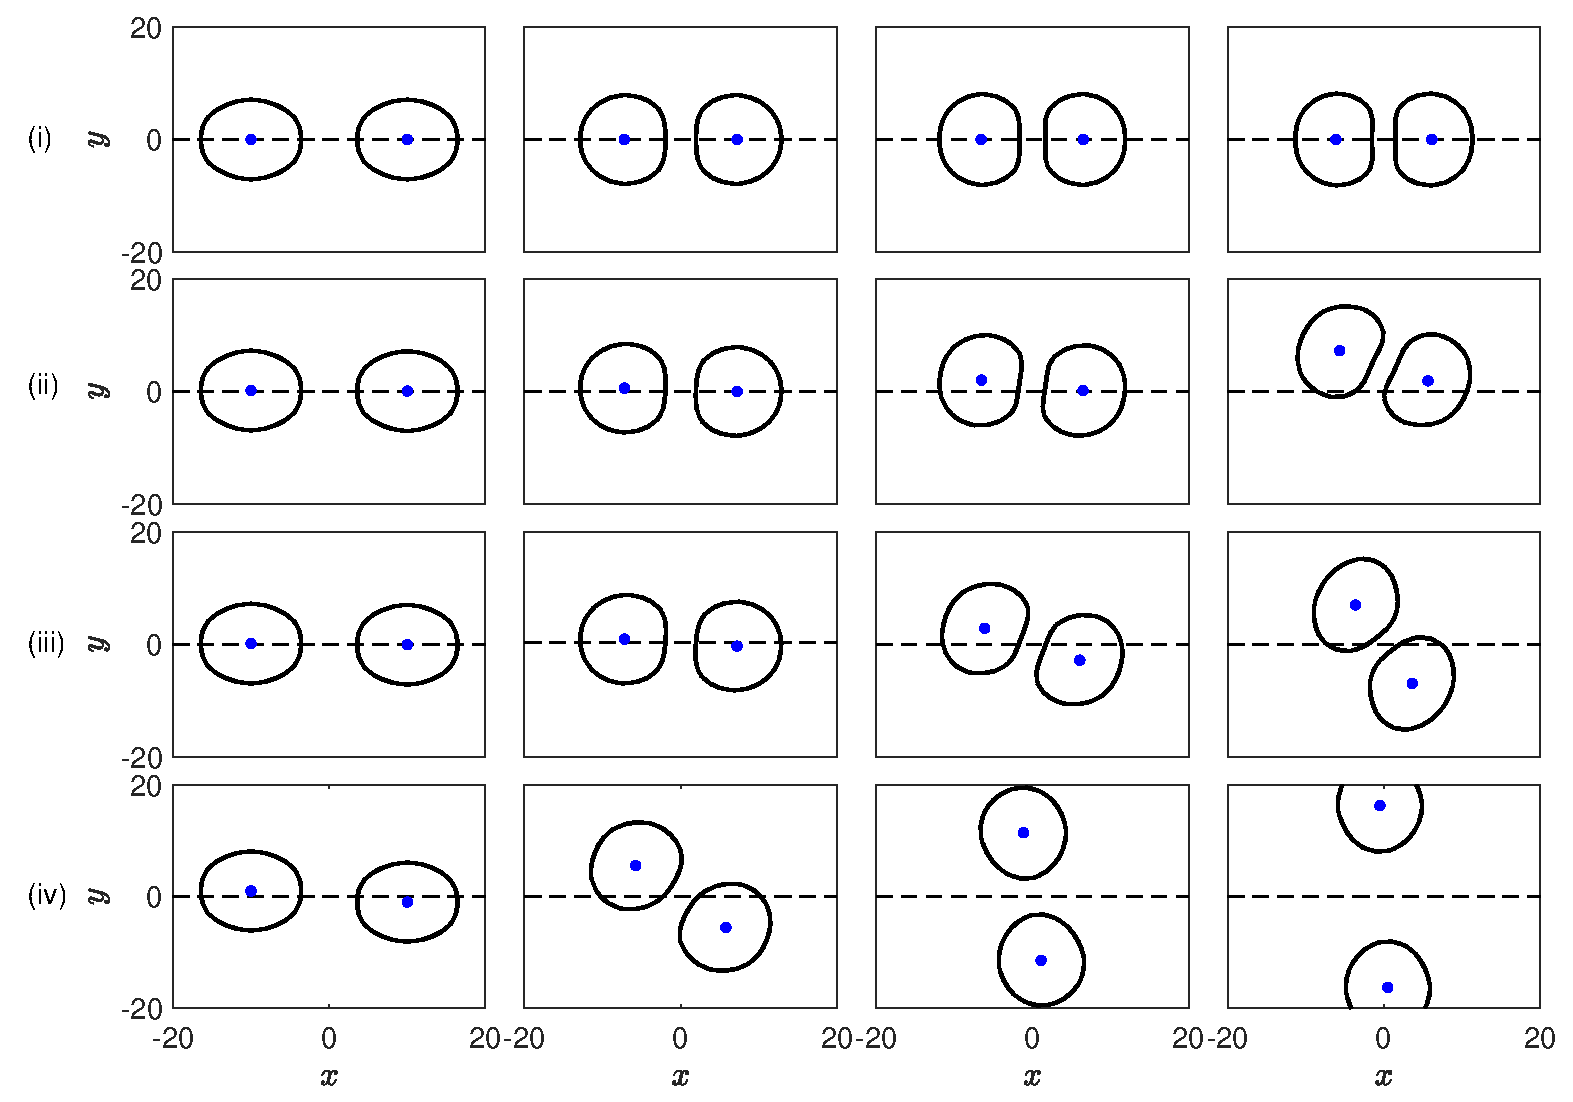
\includegraphics[width=0.9\textwidth]{ExtTraj.eps}
\end{center} 
  \caption{\label{figure11} The initial placement of two JP vesicles
  suspended in an extensional flow affects the long-time dynamics. The
  moving paths of the two centroids are plotted in blue in red. Each row
  corresponds to a different initial placement of the JP vesicles. (i)
  Both JP vesicle centroids are on the $x$-axis. (ii) The centroid of
  the left JP vesicle is $0.25$~nm above the $x$-axis and the right JP
  vesicle is on the $x$-axis. (iii) The centroid of the left JP vesicle
  is $0.25$~nm above the $x$-axis and the right JP vesicle is $0.25$~nm
  below the $x$-axis. (iv) The centroid of the left JP vesicle is
  $1.25$~nm above the $x$-axis and the centroid of the right JP vesicle
  is $1.25$~nm below the $x$-axis. The streamlines appear in grey and
  the flow rate is $\dot \gamma =0.005$~ns$^{-1}$ in all cases.}
\end{figure}


\begin{figure}
  \centering
  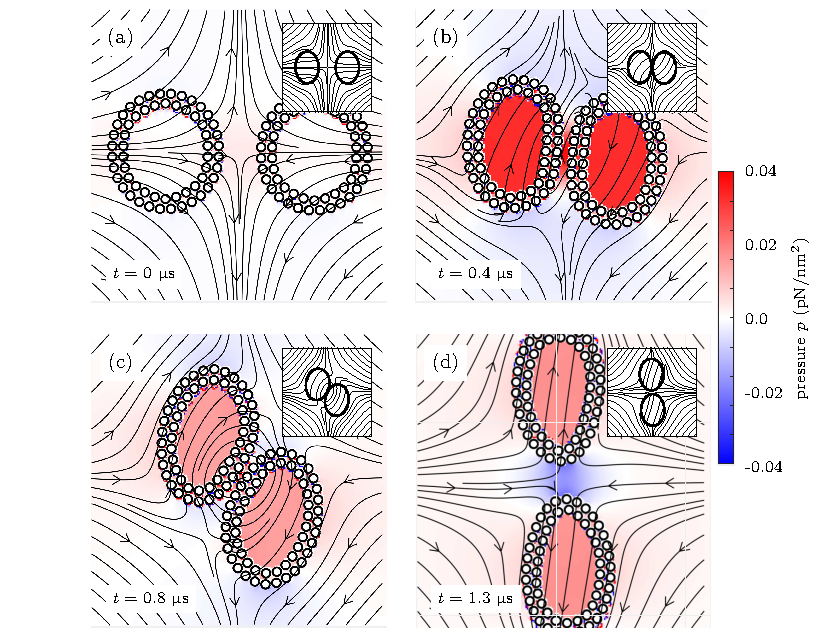
\includegraphics[width=\textwidth]{Figure12_Wrapper.pdf}
%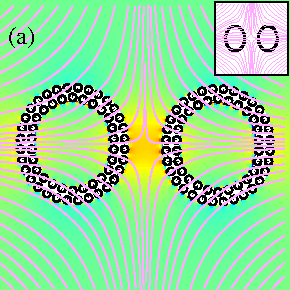
\includegraphics[height=2in]{N116_ext_0.pdf}
%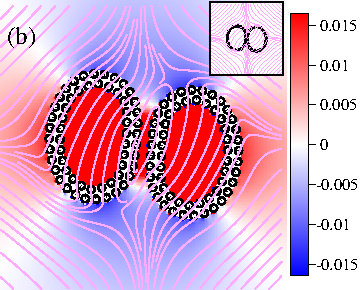
\includegraphics[height=2in]{N116_ext_2000.pdf}\\
%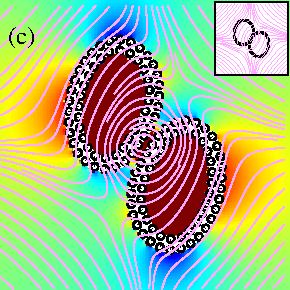
\includegraphics[height=2in]{N116_ext_4000.pdf}
%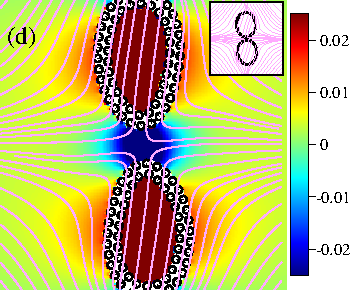
\includegraphics[height=2in]{N116_ext_6500.pdf}
  \caption{\label{figure12} The figure is for the simulation case (iii) of Figure~\ref{figure11},
  and additionally plots the pressure $p$.  The color bar is shared by all panels. 
  The insets of all panels are generated from simulations of a continuum
  model of the vesicles and the streamlines agree between the two models.}
\end{figure}





%%%%%%%%%%%%%%%%%%%%%%%%%%%%%%%%%%%%%%%%%%%%%%%%%%%%%%%%%%%%%%%%%%%%%%%
\subsubsection{Extensional Flow}

Using a similar setup to the shear flow case, we suspend the same two,
pre-relaxed, $58$-body JP vesicles and consider their dynamics in an
extensional flow 
\begin{equation}
\uu_{\infty}(\xx) = \dot \gamma ((\mathbf{e}_x \cdot \xx)\mathbf{e}_x - (\mathbf{e}_y \cdot \xx)\mathbf{e}_y)
\end{equation}
with extensional rate $\dot \gamma =0.005$ ns$^{-1}$. This extensional
flow is stretching in the $y$-direction and squeezing in the
$x$-direction. Figure~\ref{figure11} shows how the initial placement of
the JP vesicles affects the dynamics. When two centroids are both placed
symmetrically on the $x$-axis (case (i)), the JP vesicles come into
contact and reach a steady equilibrium. If one centroid is placed above
the $x$-axis (case (ii)), the two JP vesicle move together and then
upward. The migration of the right JP vesicle is a consequence of the
adhesive effect caused by the hydrophobic interactions. When the two
centroids start on opposite sides of the $x$-axis (case (iii)), they
eventually diverge from one another along the $\pm y$-directions.
Finally, when the two centroids start on opposite sides of the $x$-axis,
but with a greater displacement (case (iv)), the JP vesicles move much
faster along the $\pm y$-directions.

Figure~\ref{figure12} shows numerical results when the centroids of the
two Janus particles are placed at $(-10,-0.1)$~nm and $(10,0.1)$~nm
(case (iii) from Figure~\ref{figure11}). With this setup, the two JP
vesicles eventually separate along the $\pm y$-directions and we compare
the results against a continuum model as shown in all insets. Panels
(b)--(d) show the transient behaviour of the JP vesicles and the
continuum vesicles under an extensional flow. In both the coarse-grained
model and the continuum model, the vesicles initially converge towards
one other and then diverge along the $y$-axis. The behaviour of the
streamlines in both cases are similar. The pressure is initially largest
in the gap formed by two JP vesicles and decreases during the
separation. The short-range repulsion plays an important role to avoid
particle collisions.
%and this result can be
%compared with some findings in continuum modeling simulations. 

%may need to add more here



\begin{figure}
  \centering
  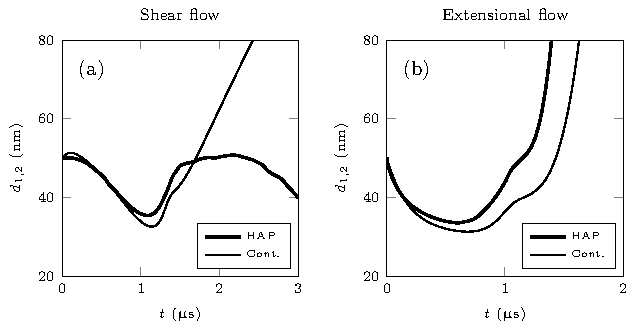
\includegraphics[width=\textwidth]{Figure13_Wrapper.pdf}
  \caption{\label{figure13} Comparisons between the proposed model and a conitnuum model in 
  two JP vesicle simulations. 
  $d_{1,2}$ is the distance between two centroids of JP vesicles. The thick curves plot the trajectories
  of $d_{1,2}$ generated by the continuum model and the thin curves are computed from using
  the proposed model.}
\end{figure}


\ReviewerOne{Since the behavior of the suspended JP vesicles has similarities to the numerical 
results generated by using the algorithm adopted in \cite{qua-vee-you2019} (refer to all figure
insets in Figure~\ref{figure10} and Figure~\ref{figure12}). Figure~\ref{figure13} shows 
trajectory comparisons between the proposed model and the continuum modeling for both 
shear flow and extensional flow cases in two vesicle simulations. The quantity $d_{1,2}$
represents the distance between two centroids of JP vesicles. The centroid positions are 
identical for both models and the geometry in the continuum model is created along the 
midplane locations of JP vesicles and the initial reduced area is matched. Panel (a) shows that 
the results of continuum model does not have a periodic motion and two vesicles flow apart 
after 1.5 $\mu$s. Panel (b) shows that the results of continuum model has similar trend of
dynamics with one in the proposed model.}



%\newpage
%%%%%%%%%%%%%%%%%%%%%%%%%%%%%%%%%%%%%%%%%%%%%%%%%%%%%%%%%%%%%%%%%%%%%%%
\section{\label{conclusion}Conclusion}

\cite{Fu20} developed a mathematical model to quantify the macroscopic
assembly and mechanics of a JP vesicle in a viscous solvent. The
interactions between JP are formulated as a second-kind integral
equation, which is coupled to the Stokes equations for the surrounding
incompressible fluid at the zero-Reynolds-number limit. Numerical
simulations of a JP suspensions revealed self-assembly of JP into
micelles and bilayers, providing an alternative means for computing
mechanical moduli, which often requires the knowledge of an equation of
state from experiments on a colloidal
membrane~(\cite{Balchunas2019_SM}).
%
%This study presents a coarse-grained model for JP vesicles that focuses
%on the hydrophobic interactions between coarse-grained lipids and
%hydrodynamic interactions. In contrast to molecular dynamic simulations,
%the hydrophobic interactions exhibit the self-assembly property of the
%lipid bilayer membrane. The proposed energy potential combined with the
%mobility problem for rigid body motions captures membrane mechanics
%including deformations, stretching modulus, and permeability of a JP
%membrane. 
%
Results in this work show great potential to study Janus colloids~(\cite{Bradley2017,Mallory2017}) and the morphology of colloid
surfactants~(\cite{Bradley2016}). 
%
%This work is highly applicable with fields in material science
%and condensed matter physics such as Janus
%colloids~(\cite{Bradley2017,Mallory2017}) and the setup can be tuned to
%match experimental results such as the morphology of colloid
%surfactants~(\cite{Bradley2016}). 
%%
For example, with the flexibility of the model, we can specify the
boundary condition on JP surfaces based on the chemicals used in
experiments.
%This can be an assist to study of interparticle interactions and chemical compositions in industry.

%Integral equation methods are used to solve the mobility problem and the
%previously introduced HAP model. We describe a method to calculate the
%hydrophobic forces and torques on each individual rigid body that avoids
%singular integrals. In addition to the HAP forces and torques, we use a
%short-range repulsion to avoid unphysical contact. 

In the present study, we used this integral formulation and numerical
algorithm to simulate the hydrodynamics of JP vesicles in background
flows. Under a linear shear flow, we found a JP vesicle to exhibit
elongation and tank-treading dynamics observed for a lipid bilayer GUV.
%
%With the use of suitable parameters, the
%numerical results yield qualitative phenomena such as a tank-treading JP
%vesicle. 
%
The results showed that the reduced area $A^*$ decreases with shear rate
but that the total length of a JP vesicle is conserved. The decay rate
of the reduced area was independent of the shear rate values between
$0.003$~ns$^{-1}$ and~$0.005$~ns$^{-1}$. Moreover, the proposed model
describes membrane rupture in high shear rates. Therefore, our method
can be applied to vesicles undergoing topological changes which is
difficult to simulate when using a continuum model that represents
vesicles as closed and continuous curves.
%
%Our coarse-grained model is also able to calculate inter-monolayer
%friction. 
%

%
%Our method requires
%calculations of the hydrodynamic stress tensor, and these are used to
%
We estimated the inter-monolayer friction $b$, membrane permeability
constant $P$, and the membrane stretching modulus $K_A$. The
inter-monolayer friction coefficient was determined by calculating the
tangential shear force and slip velocities with respect to the bilayer
mid-plane. The range of friction coefficients agree with values reported
by~\cite{denOtter2007} in their MD study. The coarse-graining level of
the JP vesicle has a larger length scale than molecular dynamics
simulations, and in the future convergence studies we will investigate
how physical properties like the friction coefficient and membrane
permeability depend on the particle shape and size.

We also simulate the spatial migration of a JP vesicle in a parabolic
shear flow. 
%The chosen parameter values result in an asymmetric
%slipper shape. 
%
Replicating the hydrodynamics of a GUV in a Poiseuille
flow~(\cite{Kaoui09, dan-vla-mis2009, cou-kao-pod-mis2008}), the JP
vesicle moves toward the centre of the shear flow. While the initial
reduced area of the JP vesicle is $A^* \approx 1$, the equilibrium
reduced area is $A^*=0.9$. For the parameters we used in the simulation,
the JP vesicle takes on an asymmetric, ``slipper" shape as it settles
above the centre of flow and exhibits tank-treading motion.
%A qualitative
%agreement is made by comparing the JP vesicle shape with the
%two-dimensional inextensible membrane in continuum modeling
%simulations~(\cite{Kaoui09, dan-vla-mis2009, cou-kao-pod-mis2008}). 
An interesting result contrast with continuum results is that the JP
vesicle oscillates at a height slightly above the centre of the
Poiseuille flow. 

%The single JP vesicle simulations end with obtaining JP bilayer stretching 
%modulus $K_A$ and hydraulic permeability constant $P$. We extract these 
%physical quantities from the Laplace pressure relationship that $R\Delta P$ is 
%proportional to JP bilayer stretch. We describe the aqueous flux in membrane 
%using a differential equation~\ref{eq:perm} and solve for the theoretical 
%permeability constant $P$. In spite of producing these values with some discrepancy
%using the default parameter set, we provide a new framework in measuring coarse-grained 
%membrane permeability.

We further simulated the hydrodynamics of two JP vesicles, and drew
comparisons with simulation results of two vesicles described by the
Helfrich continuum model. A comparison of the vesicle shapes and the
streamlines demonstrate remarkable similarities. The two overlapping
trajectories of the JP vesicles' centroids in a shear flow evolve as
expected when the two centroids are initialized on the same horizontal
level. We also observe a rotating behaviour that is observed for models
involving vesicle adhesion~(\cite{qua-vee-you2019}). The hydrophobic
attraction led to this adhesive effect when two JP bilayers are
sufficiently close. We also performed several simulations of a pair of
JP vesicles suspended in an extensional flow. By varying the initial
vertical displacement of the vesicles' centroids, we can control for
divergent trajectories and obtain similar results to the continuum
model.

In \S~\ref{subsec:calculating_force}, we derived an alternative integral
form for calculating the force and torque to avoid the singular integral
evaluation. These alternative integrals allow us to accurately resolve
trajectories over long times without having to rely on computationally
expensive quadratures.

Our future goals include extending the current framework to a
three-dimensional JP vesicle system. This will require additional
algorithmic implementation including a fast summation method such as the
fast multipole method. Another research direction is to include the
fluctuating hydrodynamics for Brownian suspensions~(\cite{Bao2018}),
%introduce thermal fluctuations into the model. 
%This will result in Janus particles that include Brownian motion, 
and this is critical to understand membrane diffusion. Finally, a more
physical boundary conditions for the HAP model will allow us to draw
comparisons between computational and laboratory experiments.


\begin{acknowledgments}
  {\bf Acknowledgments:} B.Q.~acknowledges support from NSF (Grant
  No.~DMS 2012560) and from the Simons Foundation, Mathematics and
  Physical Sciences-Collaboration Grants for Mathematicians (Award
  No.~527139). Y.-N. Y.~acknowledges support from NSF (Grant No.~DMS 1614863 and 1951600) and
  Flatiron Institute, part of Simons Foundation.
%We would like to acknowledge 
\end{acknowledgments}

%\appendix
%
%\section{Appendices}
%\label{sec:appendixA}

\bibliographystyle{jfm}
\bibliography{reference}% Produces the bibliography via BibTeX.

% Supplementary Materials

\thispagestyle{empty}

\newpage
{\Large \bf

  \noindent Supplementary Material\\

  \noindent 
 Effects of Tunable Hydrophobicity on the Collective Hydrodynamics of Janus Particles under Flows}\\

\noindent 
Szu-Pei Fu$^{1,*},$ 
Rolf Ryham$^{2},$ 
Bryan Quaife$^{3}$ and Y.-N. Young$^{4},$
\\

\noindent
$^{1}$Department of Mathematics, Trinity College, Hartford, Connecticut 06106, USA

\noindent
$^{2}$Department of Mathematics, Fordham University, Bronx, NY, USA

\noindent
$^{3}$Department of Scientific Computing, Florida State University, Tallahassee, Florida 32306, USA

\noindent
$^{4}$Department of Mathematical Sciences, New Jersey Institute of Technology, Newark, NJ 07102 USA
\\

\noindent $^*$Corresponding author. Address: Department of Mathematics, Trinity College, 
300 Summit Street, Hartford, CT 06106. email: \text{peter.fu@trincoll.edu}



\setcounter{page}{1}

\setcounter{figure}{0}
\renewcommand{\thefigure}{S\arabic{figure}}

\setcounter{equation}{0}
\renewcommand{\theequation}{S\arabic{equation}}

\setcounter{section}{0}
\renewcommand{\thesection}{S\arabic{section}} 


%-----ellipse repulsion--------------------

%\Phi_{\mathrm{rep}}

\section{Movie Captions}\mbox{} \\

\noindent
{\bf Movie S1. Relaxation} 
There are 60 circular particles with radius 1.25~nm that are initially
confined in a square box. The simulation results show the relaxation
with each of the three boundary conditions. The time step of all
simulations is $\Delta t=0.2$. The color on the boundary from blue to
red is for $\min g(\xx)$ to $\max g(\xx)$. All final configurations are
adopted in simulations with hydrodynamic flows. \\


\noindent
{\bf Movie S2. Structures in a Shear Flow without Ruptures} 
We adopt the relaxed configurations and place the JP structures in the
shear flow. For the choices of the shear rate, we pick: $\dot\gamma =
0.05$ ns$^{-1}$ for the vesicle, $\dot\gamma = 0.05$ ns$^{-1}$ for the bilayer, $\dot\gamma
= 0.05$ ns$^{-1}$ for the multi-lamellar, and $\dot\gamma = 0.1$ ns$^{-1}$ for the striated
configurations. The vesicle case undergoes tank-treading whereas the
initially disordered BC (i) case increases orientational order. The
multilamellar assemply behaves as a rigid body, and the striated
configuration moreso. No ruptures occur. \\



\noindent
{\bf Movie S3. Structures in a Taylor-Green Flow without Ruptures} 
We adopt the relaxed configurations and place the JP structures in the
Taylor-Green flow at low flow rates. For the choices of the flow
strength, we pick: $\dot\gamma = 0.05$ ns$^{-1}$ for the vesicle, $\dot\gamma = 0.05$ ns$^{-1}$ for the
disordered bilayer, $\dot\gamma = 0.05$ ns$^{-1}$ for the multi-lamellar, and $\dot\gamma = 0.1$ ns$^{-1}$
for the striated configurations. The vesicle stays inact, whereas the
dissordered bilayer is pulled apart. Like in Supplementary Movie S2, the
striated assembly is basically rigid. \\


\noindent
{\bf Movie S4. Structures in a Shear Flow with Ruptures} 
We adopt the relaxed configurations and place the JP structures in the
shear flow at a higher shear rate. For the choices of the shear rate, we
pick: $\dot\gamma = 0.075$ for the vesicle, $\dot\gamma = 0.1$ ns$^{-1}$ for the
bilayer, $\dot\gamma = 0.15$ ns$^{-1}$ for the multi-lamellar, and $\dot\gamma =
0.15$ ns$^{-1}$ for the striated configurations. The time step of all simulations
is $\Delta t=0.2$ ns$^{-1}$. In this movie, some clear structural ruptures occur
in each case. In order to observe the structure behaviors at later time,
we stabilize the frame by tracking the center of mass position of all
JP. \\


\noindent
{\bf Movie S5. Structures in a Taylor-Green Flow with Ruptures} 
We adopt the relaxed configurations and place the JP structures in the
Taylor-Green flow at higher flow rates. For the choices of the flow
strength, we pick: $\dot\gamma = 0.1$ ns$^{-1}$ for the vesicle, $\dot\gamma = 0.1$ ns$^{-1}$ for the
bilayer, $\dot\gamma = 0.1$ ns$^{-1}$ for the multi-lamellar, and $\dot\gamma = 0.15$ ns$^{-1}$ for the
striated configurations. Clear structural ruptures occur in each case.
In all cases, there is significant reduction in the orientational order
of the assemblies. While the BC (i) cases are broken into several
pieces, the main body of the BC (ii) and BC (iii) assemblies are not
pulled apart by the background flow.\\

\noindent
{\label{MovieS6}\bf Movie S6. Single Vesicle in a Taylor-Green Flow with Various $\lambda$ Values} 
A circular vesicle bilayer is placed in the Taylor-Green flow. 
The parameter $\lambda$ controls the cell size and the values are varied from 1.0 nm to 4.0 nm while the flow rate $\lambda\dot\gamma=0.1$ is fixed. There is a rotation transition from clockwise ($\lambda=1$ nm and  2 nm) to counterclockwise ($\lambda=3$ nm and 4 nm). Moreover, the resulting steady shapes of all cases are different polygons. We plot the streamlines in the background.\\





\section{Raw Data}
The following figures plot the fully resolved simulation time-courses
organized in terms of the bilayer, vesicle BL, multilamellar, and striated JP phases
under shear flow (Supplementary Figures~\ref{fig:ulshraw}--\ref{fig:stshraw})
and under TG flow (Supplementary Figures~\ref{fig:ultgraw}--\ref{fig:sttgraw}).
Throughout, panels (a) are for relative free energy $F - F_0$,
panels (b) for alignment $S_2$, and panels (c) for strain $E$ (as a percentage). 
A common ordinate is used for each of the respective panels to facilitate
comparison between data sets. 
%\newpage

\begin{figure}[h!]
\begin{center}
\textbf{\textsc{Shear Flow cases}}\par\medskip
\textbf{Type I, bilayer phase under shear flow}\par\medskip
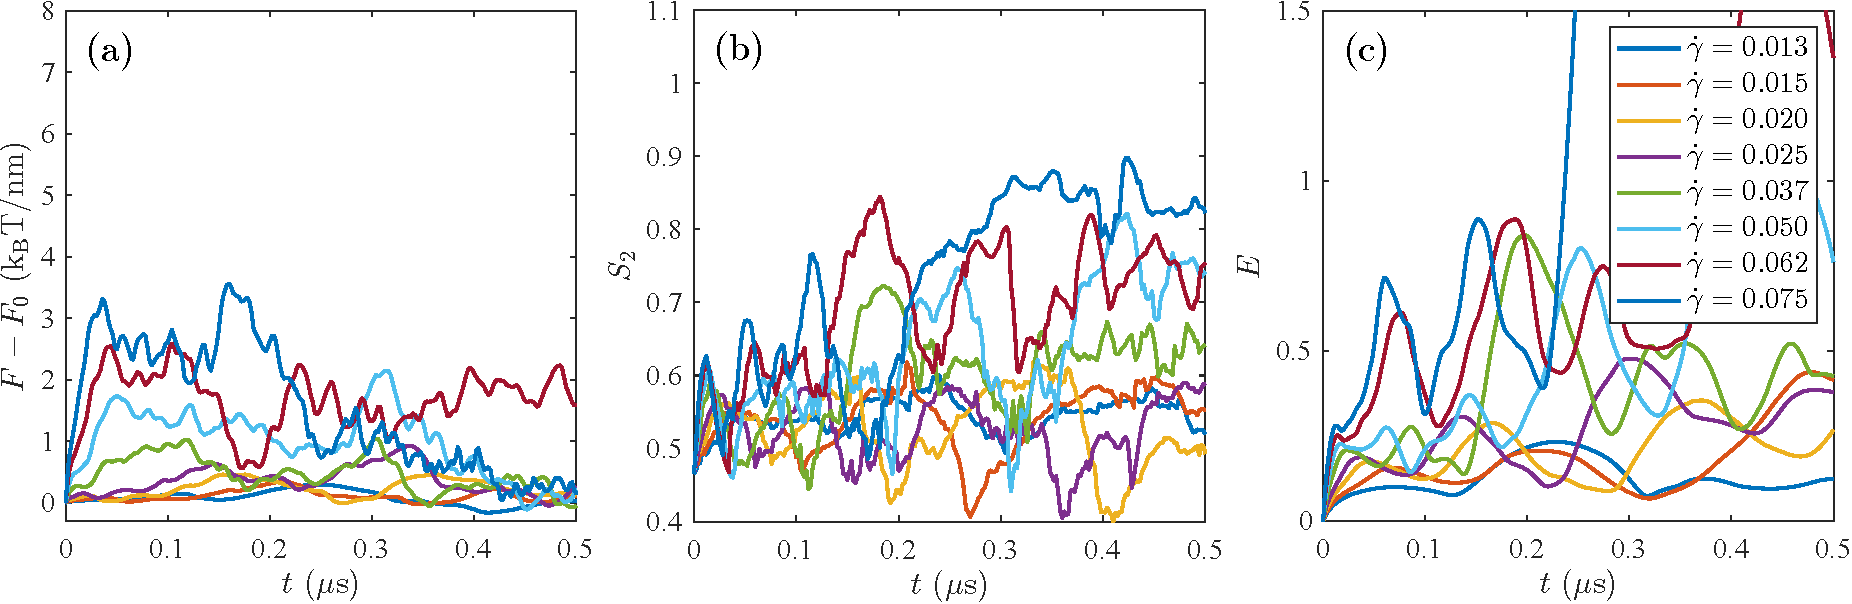
\includegraphics[width=\textwidth]{SMFigures/ULShRaw.pdf}
\end{center}
\caption{
Relative free energy $F - F_0$,
alignment $S_2$, and strain $E$ for
Type I, bilayer phase under shear flow with choices of shear rates $\dot\gamma=0.013$ -- $0.075$ ns$^{-1}$.
%The change in free energy $F$ is plotted in panel (a). Panel (b) shows the scalar order parameter $S_2$ over time $t$. Panel (c) plots the change of strain parameter $E$ in percentage over time $t$.
}
\label{fig:ulshraw}
\end{figure}


\begin{figure}[h!]
\begin{center}
\textbf{Type I, vesicle BL phase under shear flow}\par\medskip
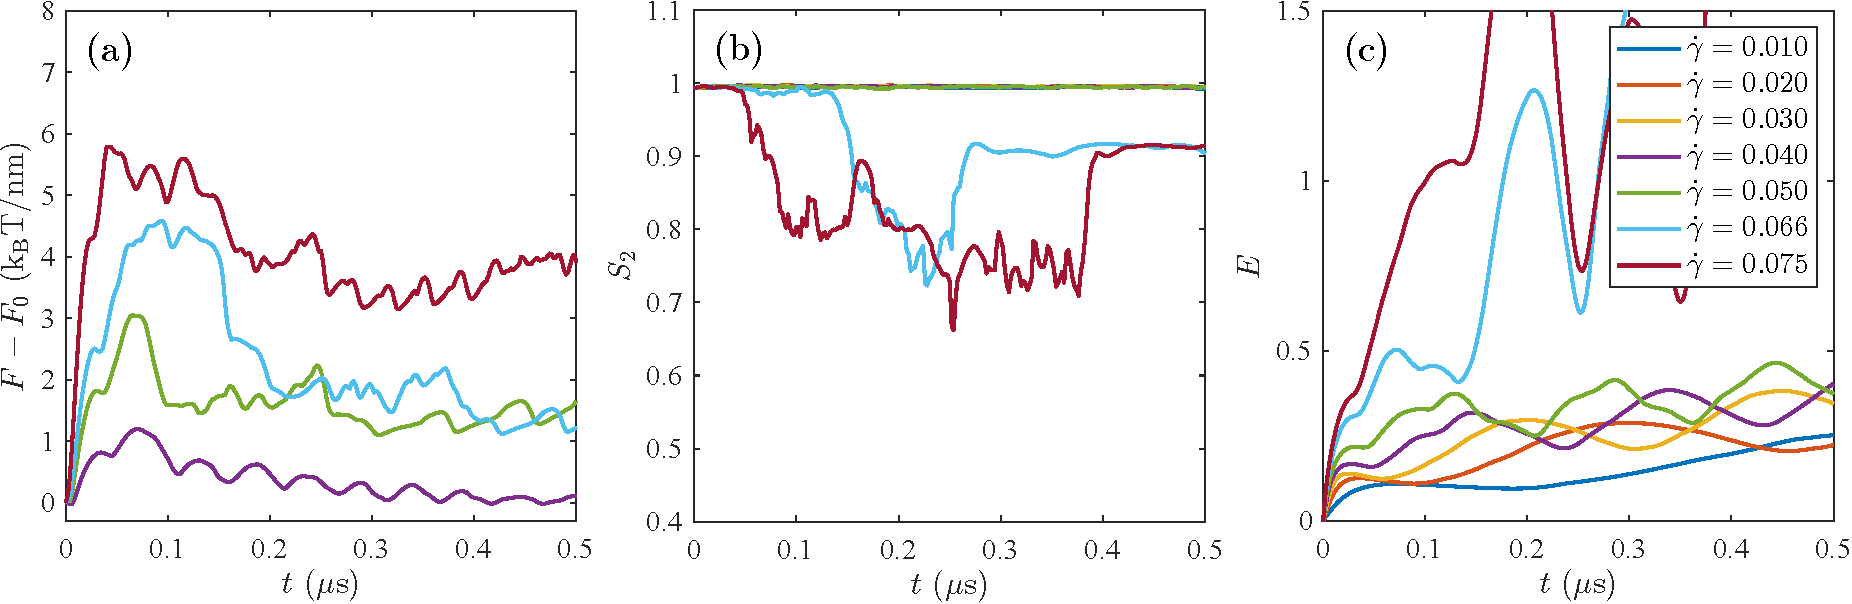
\includegraphics[width=\textwidth]{SMFigures/VeShRaw.pdf}
\end{center}
\caption{
Relative free energy $F - F_0$,
alignment $S_2$, and strain $E$ for
Type I, bilayer phase under shear flow with choices of shear rates $\dot\gamma=0.01$ -- $0.075$ ns$^{-1}$.
The JP type is the same as for Supplementary Figure \ref{fig:ulshraw} but with a
ring-shaped, rather than disordered, bilayer for initial configuration.  
%A Vesicle under a shear flow with choices of shear rates $\dot\gamma=0.01\sim0.075$. The change in free energy $F$ is plotted in panel (a). Panel (b) shows the scalar order parameter $S_2$ over time $t$. Panel (c) plots the change of strain parameter $E$ in percentage over time $t$.
}
\label{fig:veshraw}
\end{figure}


\begin{figure}[h!]
\textbf{Type II, multilamellar phase under shear flow}\par\medskip
\begin{center}
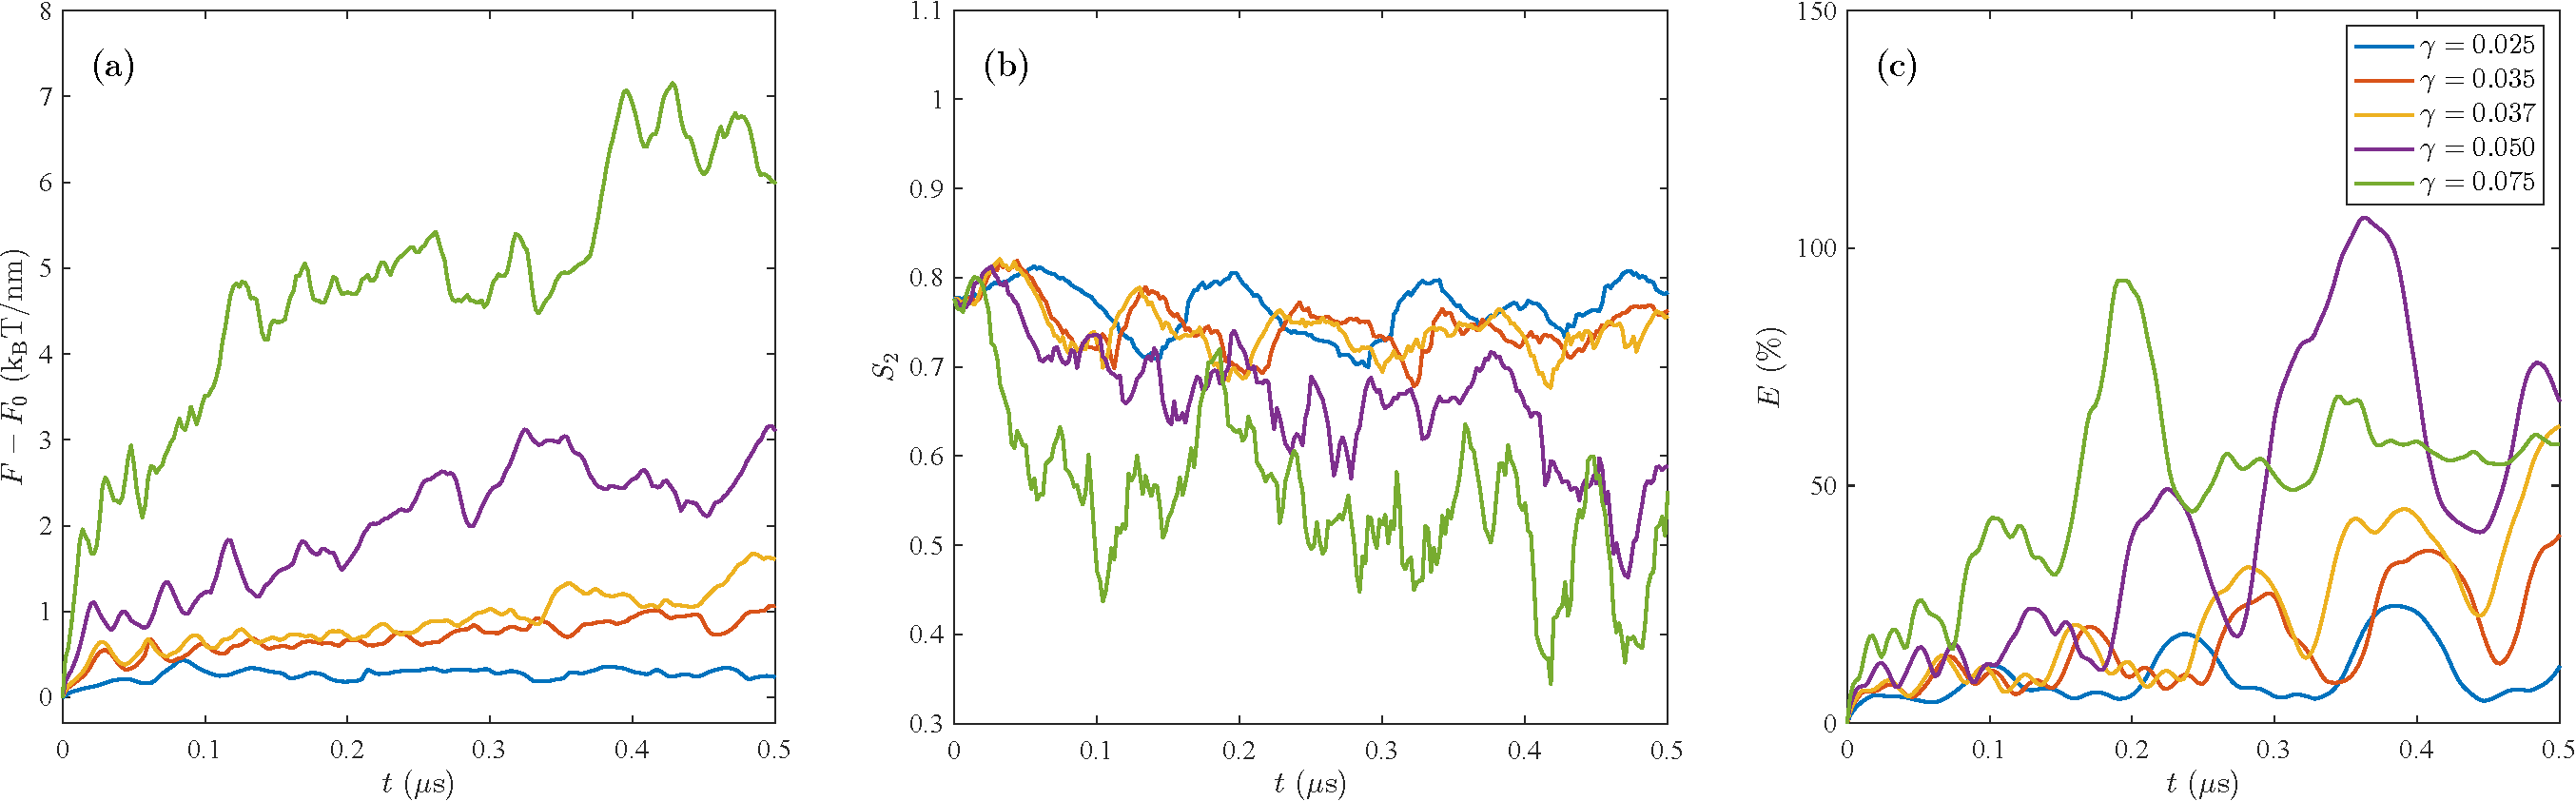
\includegraphics[width=\textwidth]{SMFigures/MLShRaw.pdf}
\end{center}
\caption{
Relative free energy $F - F_0$,
alignment $S_2$, and strain $E$ for
Type II, multilamellar phase under shear flow with choices of shear rates $\dot\gamma=0.025$ -- $0.075$ ns$^{-1}$.
%A multilamellar JP structure under a shear flow with choices of shear rates $\dot\gamma=0.025\sim0.075$. The change in free energy $F$ is plotted in panel (a). Panel (b) shows the scalar order parameter $S_2$ over time $t$. Panel (c) plots the change of strain parameter $E$ in percentage over time $t$.
}
\label{fig:mlshraw}
\end{figure}


\begin{figure}[h!]
\textbf{Type III, striated phase under shear flow}\par\medskip
\begin{center}
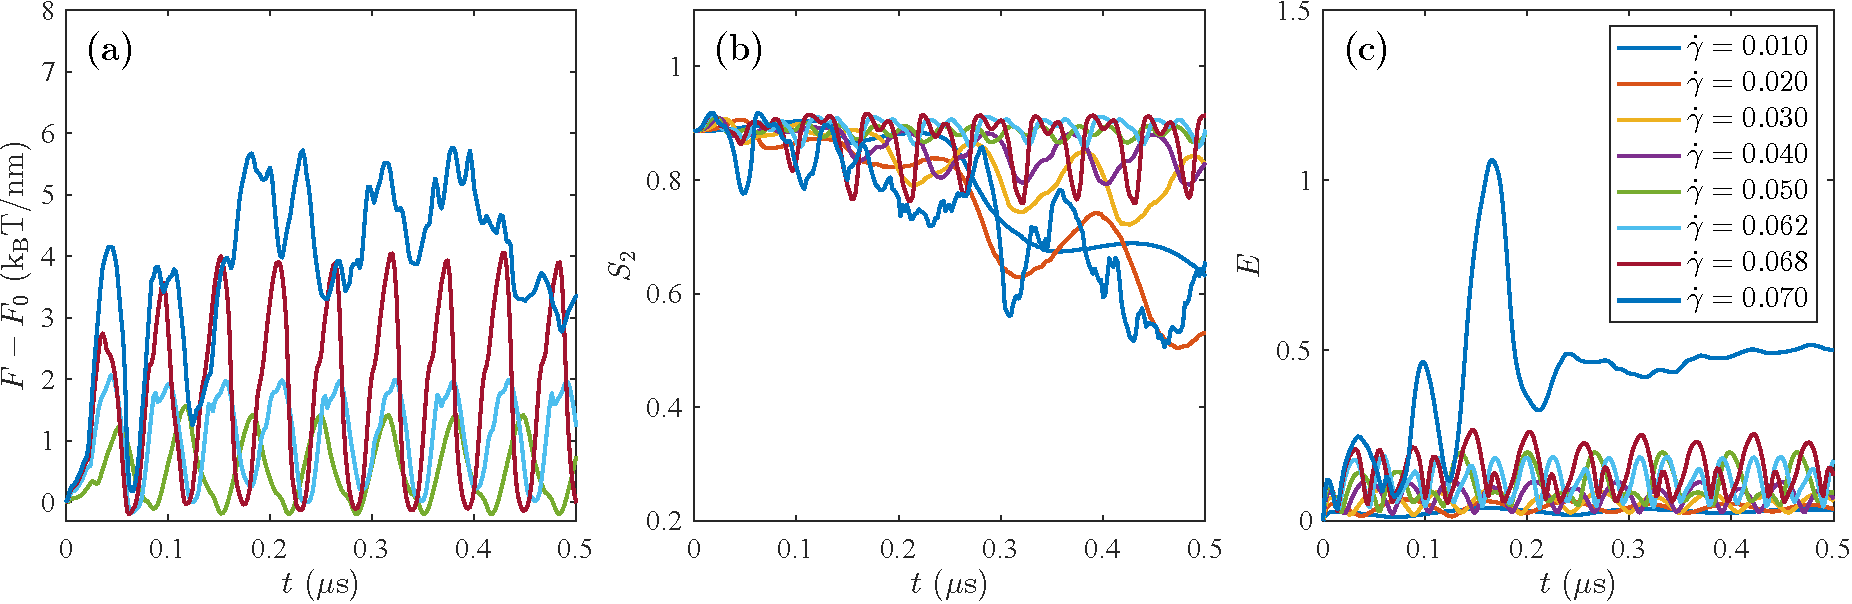
\includegraphics[width=\textwidth]{SMFigures/StShRaw.pdf}
\end{center}
\caption{
Relative free energy $F - F_0$,
alignment $S_2$, and strain $E$ for
Type III, striated phase under shear flow with choices of shear rates $\dot\gamma=0.01$ -- $0.07$ ns$^{-1}$.
%A striated JP structure under a shear flow with choices of shear rates $\dot\gamma=0.01\sim0.07$. The change in free energy $F$ is plotted in panel (a). Panel (b) shows the scalar order parameter $S_2$ over time $t$. Panel (c) plots the change of strain parameter $E$ in percentage over time $t$.
}
\label{fig:stshraw}
\end{figure}

\begin{figure}[h!]
\begin{center}
\textbf{\textsc{TG Flow Cases}}\par\medskip
\textbf{Type I, bilayer  phase under TG flow}\par\medskip
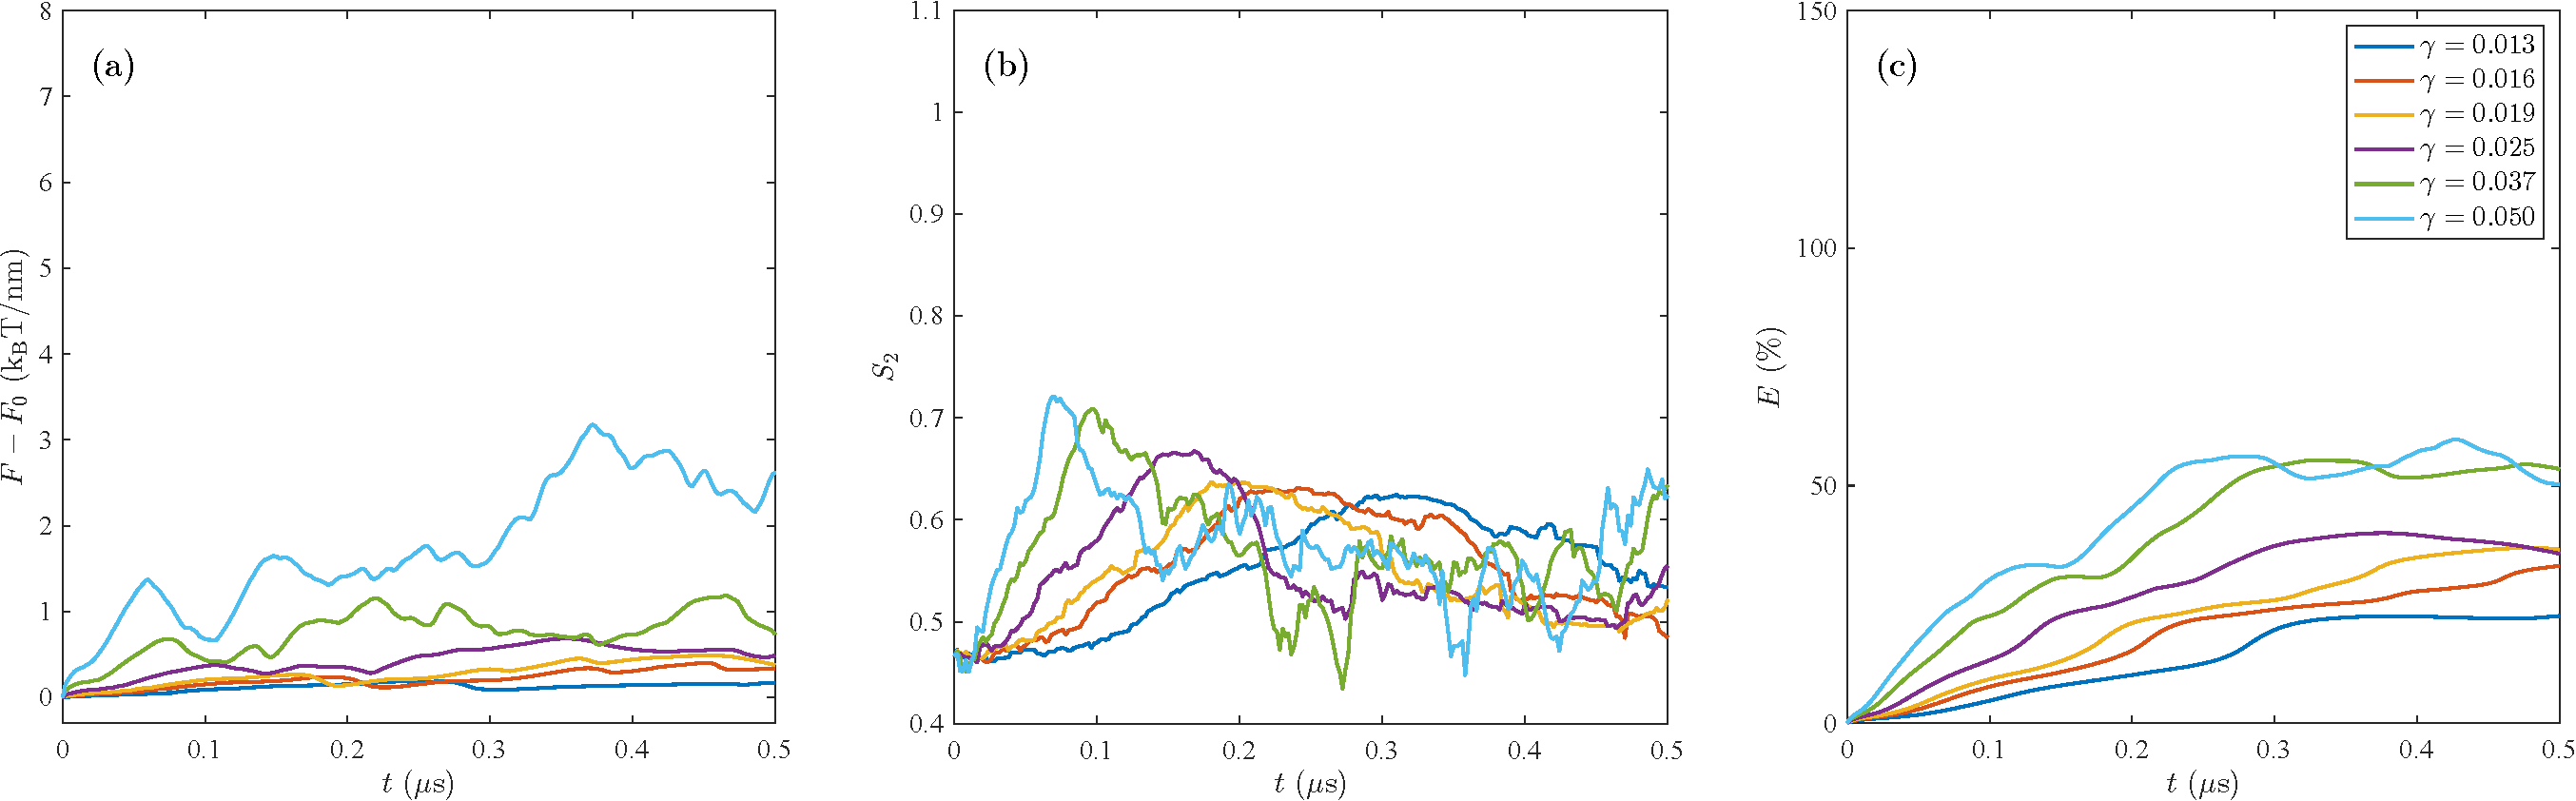
\includegraphics[width=\textwidth]{SMFigures/ULTGRaw.pdf}
\end{center}
\caption{
Relative free energy $F - F_0$,
alignment $S_2$, and strain $E$ for
Type I, bilayer phase under TG flow with choices of shear rates $\dot\gamma=0.013$ -- $0.05$ ns$^{-1}$.
%A unilamellar JP structure under a TG flow with choices of shear rates $\dot\gamma=0.013\sim0.05$. The change in free energy $F$ is plotted in panel (a). Panel (b) shows the scalar order parameter $S_2$ over time $t$. Panel (c) plots the change of strain parameter $E$ in percentage over time $t$.
}
\label{fig:ultgraw}
\end{figure}


\begin{figure}[h!]
\begin{center}
\textbf{Type I, vesicle BL phase under TG flow}\par\medskip
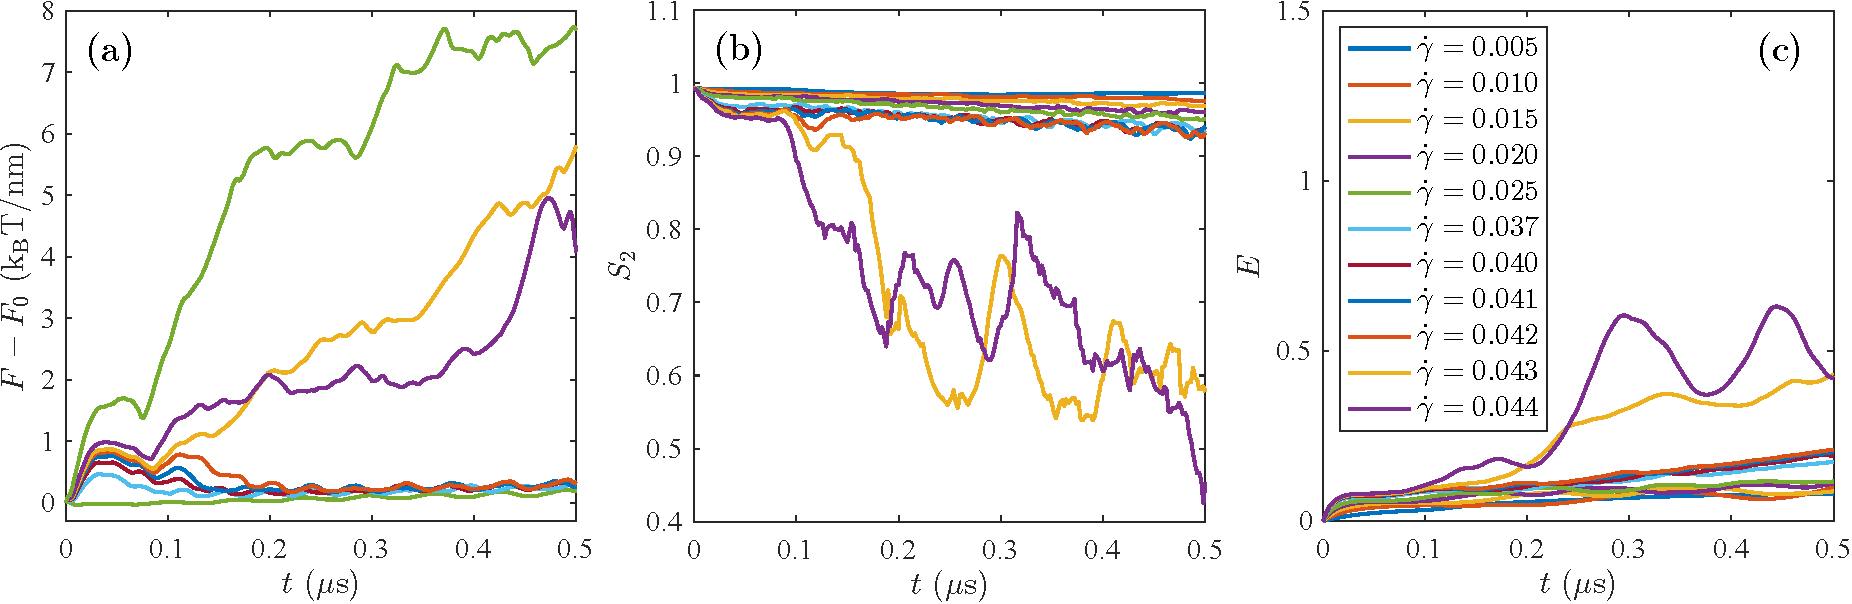
\includegraphics[width=\textwidth]{SMFigures/VeTGRaw.pdf}
\end{center}
\caption{
Relative free energy $F - F_0$,
alignment $S_2$, and strain $E$ for
Type I, vesicle bilayer phase under TG flow with choices of shear rates $\dot\gamma=0.005$ -- $0.044$ ns$^{-1}$.
The JP type is the same as for Supplementary Figure \ref{fig:ultgraw} but with a
ring-shaped, rather than disordered, bilayer for initial configuration.  
%A vesicle JP structure under a TG flow with choices of shear rates $\dot\gamma=0.005\sim0.044$. The change in free energy $F$ is plotted in panel (a). Panel (b) shows the scalar order parameter $S_2$ over time $t$. Panel (c) plots the change of strain parameter $E$ in percentage over time $t$.
}
\label{fig:vetgraw}
\end{figure}




\begin{figure}[h!]
\begin{center}
\textbf{Type II, multilamellar phase under TG flow}\par\medskip
\includegraphics[width=\textwidth]{SMFigures/MLTGRaw.pdf}
\end{center}
\caption{
Relative free energy $F - F_0$,
alignment $S_2$, and strain $E$ for
Type II, multilamellar phase under TG flow with choices of shear rates $\dot\gamma=0.025$ -- $0.069$ ns$^{-1}$.
%A multilamellar JP structure under a TG flow with choices of shear rates $\dot\gamma=0.025\sim0.069$. The change in free energy $F$ is plotted in panel (a). Panel (b) shows the scalar order parameter $S_2$ over time $t$. Panel (c) plots the change of strain parameter $E$ in percentage over time $t$.
}
\label{fig:mltgraw}
\end{figure}


\begin{figure}[h!]
\begin{center}
\textbf{Type III, striated phase under TG flow}\par\medskip
\includegraphics[width=\textwidth]{SMFigures/StTGRaw.pdf}
\end{center}
\caption{
Relative free energy $F - F_0$,
alignment $S_2$, and strain $E$ for
Type III, striated phase under TG flow with choices of shear rates $\dot\gamma=0.01$ -- $0.075$ ns$^{-1}$.
%A striated JP structure under a TG flow with choices of shear rates $\dot\gamma=0.01\sim0.069$. The change in free energy $F$ is plotted in panel (a). Panel (b) shows the scalar order parameter $S_2$ over time $t$. Panel (c) plots the change of strain parameter $E$ in percentage over time $t$.
}
\label{fig:sttgraw}
\end{figure}








%\bibliographystyle{jfm}
%\bibliography{jfm}
%Use of the above commands will create a bibliography using the .bib file. Shown below is a bibliography built from individual items.


%\bibliography{jfm2esam}

%\begin{thebibliography}{99}
%
%\expandafter\ifx\csname natexlab\endcsname\relax
%\def\natexlab#1{#1}\fi
%\expandafter\ifx\csname selectlanguage\endcsname\relax
%\def\selectlanguage#1{\relax}\fi
%
%\bibitem[Batchelor (1971)]{Batchelor59}
%{\sc Batchelor, G.K.} 1971 {Small-scale variation of convected quantities like temperature in turbulent fluid part1, general discussion and the case of small conductivity}, {\it J. Fluid Mech.}, {\bf 5}, pp. 3-113-133.
%
%\bibitem [Bouguet (2008)]{Bouguet01}
%{\sc Bouguet, J.-Y} 2008 Camera Calibration Toolbox for Matlab {\url{http://www.vision.caltech.edu/bouguetj/calib_doc/}}.
%
% \bibitem[Briukhanovetal et al (1967)] {Briukhanovetal1967}
%{\sc Briukhanov, A. V.,   Grigorian, S. S., Miagkov,  S. M., Plam, M. Y.,   I. E. Shurova, I. E.,   Eglit, M. E. and Yakimov, Y. L.} 1967
%{On some new approaches to the dynamics of snow avalanches},
%{\it Physics of Snow and Ice,  Proceedings of the International Conference on Low Temperature Science}
%{Vol 1} pp. 1221--1241 {Institute of Low Temperature Science, Hokkaido University, Sapporo, Hokkaido, Japan}.
%
%\bibitem[Brownell (2004)]{Brownell04}
% {\sc Brownell,  C.J.  and Su,  L.K.} 2004  {Planar measurements of differential diffusion in turbulent jets}, {\it AIAA Paper},  pp. 2004-2335.
%
%\bibitem[Brownell and Su (2007)] {Brownell07}
%  {\sc Brownell, C.J. and  Su, L.K.} 2007 {Scale relations and spatial spectra in a differentially diffusing jet}, {\it AIAA Paper}, pp 2007-1314.
%
%\bibitem [Dennis (1985)] {Dennis85}
% {\sc  Dennis, S.C.R.} 1985 {Compact explicit finite difference approximations to the Navier--Stokes equation},  { In \it Ninth Intl Conf. on Numerical Methods in Fluid Dynamics},  {ed Soubbaramayer and J.P. Boujot},  {Vol 218}, {\it Lecture Notes in Physics}, pp. 23-51. Springer.
%
%\bibitem [Edwards et al. (2017)]{EdwardsVirouletKokelaarGray2017}
%{\sc Edwards, A. N., Viroulet, S., Kokelaar, B. P. and Gray, J. M. N. T.} 2017 Formation of levees, troughs and elevated channels by avalanches on erodible slopes {\it J. Fluid Mech.}, {\bf 823}, pp. 278-315.
%
%\bibitem[Hwang et al (1970)] {Hwang70}
% {\sc Hwang,  L.-S.  and  Tuck, E.O.} 1970 On the oscillations of harbours of arbitrary shape {\it J.~Fluid Mech.}, {\bf42}, pp 447-464.
%
%\bibitem[Josep and Saut (1990)] {JosephSaut1990}
% {\sc Joseph, Daniel D. and Saut, Jean Claude} 1990 Short-wave instabilities and ill-posed initial-value problems {\it Theoretical and Computational Fluid Dynamics}, {\bf 1},  pp.191--227,  {\url{http://dx.doi.org/10.1007/BF00418002}}.
%
%\bibitem[Worster (1992)] {Worster92}
%{ \sc  Worster, M.G.} 1992 The dynamics of mushy layers {\it Interactive dynamics of convection and solidification},
%{(ed. S.H. Davis and H.E. Huppert and W. Muller and M.G. Worster)}, pp. 113--138 {Kluwer}.
%
%\bibitem[Koch(1983)] {Koch83}
%{\sc Koch, W.} 1983 Resonant acoustic frequencies of flat plate cascades {\it J.~Sound Vib.}, {\bf 88}, pp. 233-242.
%
%\bibitem[Lee(1971)] {Lee71}
%{\sc Lee,  J.-J.}  1971 Wave-induced oscillations in harbours of arbitrary geometry {\it J.~Fluid Mech.}, {\bf 45}, pp. 375-394.
%
%\bibitem[Linton and  Evans (1992)] {Linton92}
% {\sc  Linton, C.M. and  Evans, D.V.} 1992 The radiation and scattering of surface waves by a vertical circular cylinder in a channel {\it Phil.\ Trans.\ R. Soc.\ Lond.}, {\bf 338}, pp. 325-357.
%
%\bibitem [Martin(1980] {Martin80}
% {\sc  Martin, P.A.} 1980 On the null-field equations for the exterior problems of acoustics {\it Q.~J. Mech.\ Appl.\ Maths},{\bf 33}, pp. 385--396.
%
%\bibitem [Rogallo(1981)] {Rogallo81}
% {\sc Rogallo,  R.S.} 1981 Numerical experiments in homogeneous turbulence  { {\it Tech. Rep.} 81835}  {NASA Tech.\ Mem}.
%
%\bibitem[Ursell(1950)] {Ursell50}
%{\sc  Ursell, F.} 1950 Surface waves on deep water in the presence of a submerged cylinder i {\it Proc.\ Camb.\ Phil.\ Soc.}, {\bf 46}, pp.141--152.
%
%\bibitem[Wijngaarden (1968)]{Wijngaarden68}
%{\sc van Wijngaarden, L.} 1968 On the oscillations Near and at resonance in open pipes {\it J.~Engng Maths},{\bf 2}, pp. 225--240.
%
%\bibitem[Miller (1991)]{Miller91}
%{ \sc  Miller, P.L.} 1991 Mixing in high Schmidt number turbulent jets {school {PhD thesis}} {California Institute of Technology}.
%
%\end{thebibliography}

%% End of file `jfm2esam.bib'.

\end{document}
